\documentclass{article}

% Formatting
\usepackage[utf8]{inputenc}
\usepackage[margin=1in]{geometry}
\usepackage[titletoc,title]{appendix}
\usepackage[spanish]{babel}
\usepackage{amsmath,amsfonts,amssymb,mathtools}
\usepackage{graphicx,float}
\usepackage[ruled,vlined]{algorithm2e}
\usepackage{algorithmic}
\usepackage{minted}
\usemintedstyle{borland}
\usepackage{subcaption}
\usepackage{multicol}
\usepackage{listings}
\usepackage{xcolor}
\usepackage{biblatex}
\addbibresource{ref.bib}
\usepackage{minted}



% Title content
\title{Práctica 7 búsqueda local}
\author{Denisse Leyva}
\date{Abril 14, 2021}

\begin{document}

\maketitle


\section{Introducción}
En la séptima práctica implementamos una optimización heurística sencilla para encontrar máximos locales de funciones, los ejemplos siendo de Womersley\cite{Rob_Womersley} los matemáticamente inclinados pueden consultar su trabajo por métodos de búsqueda más sofisticados, guiados por métodos matemáticos de mayor rigor.

Buscamos minimizar la función unidimensional, a partir de un punto seleccionado al azar, realizando movimientos locales. Estando en $x$ se seleccionará al azar un $\Delta x > 0$  pequeño, calculará los valores $f(x \pm \Delta x)$ y seleccionará el menor de los dos como el siguiente valor de $x$. Esto se repite $k$ veces y aquel $x$ que produjo el menor valor de $f(x)$ se regresa como el resultado. Se realizarán $n$ réplicas y el menor de ellos es el resultado de la búsqueda en sí \cite{Satu_Elisa_Schaeffer}.

\section{Objetivo}
La tarea se trata de maximizar algún variante de la función bidimensional ejemplo $g(x,y)$ con restricciones $-3\leq x, y \leq 3$, con la misma técnica del ejemplo unidimensional. La posición actual es un par $x , y$ y se ocupan dos movimientos aleatorios, $\Delta x$ y $\Delta y $, cuyas combinaciones posibles proveen ocho posiciones vecino, de las cuales aquella que logre el mayor valor para $g$ es seleccionado \cite{Satu_Elisa_Schaeffer}.
Dibujado en tres dimensiones, $g(x,y)$  se ve así

\begin{figure}[H]
\centering
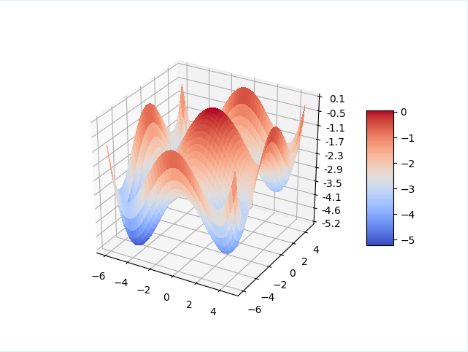
\includegraphics[width=100mm]{figura_objetivo.png}
\caption{\label{fig3} Gráfica 3D de ejemplo.} 
\end{figure}

\section{Código}
Para este código se tomó en cuenta las 8 posiciones en combinación a los puntos cardinales de la posición inicial, también se tuvo que poner un limitante para que los agentes no se salgan de los límites.
Para escoger el mayor se guardaron todos los resultados de las 8 posiciones en una lista de la cual se agarra la posición del mayor y modificamos la posición con el selector. Se utilizó el código base de Schaeffer \cite{Elisa_Schaeffer} para obtener la visualización en una proyección en el plano $x , y$. El código completo esta en GitHub \cite{Denisse_Leyva}.
\renewcommand{\listingscaption}{Código}
\begin{listing}[H]
  \begin{minted}[linenos,mathescape,texcl]{clojure}
r = agentes.iloc[i]
xl = r.x - r.dx
xr = r.x + r.dx
yd = r.y - r.dy
yu = r.y + r.dy
if  xl < low+step:
    xl = r.x
if  xr > high-step:
    xr = r.x
if  yd < low+step:
    yd = r.y
if  yu > high-step:
    yu = r.y
g1 = g(xl, yu)
g2 = g(r.x, yu)
g3 = g(xr, yu)
g4 = g(xl, r.y)
g5 = g(xr, r.y)
g6 = g(xl, yd)
g7 = g(r.x, yd)
g8 = g(xr, yd)
lista = [g1,g2,g3,g4,g5,g6,g7,g8]
mayor = lista.index(max(lista))+1   
if mayor == 1:
    agentes.at[i, 'x'] = xl
    agentes.at[i, 'y'] = yu
elif mayor ==2:
    agentes.at[i, 'x'] = r.x
    agentes.at[i, 'y'] = yu
elif mayor ==3:
    agentes.at[i, 'x'] = xr
    agentes.at[i, 'y'] = yu
...
    \end{minted}
  \label{lst:fibo}
  \caption{Realiza el movimiento de los agentes.}
\end{listing}

\section{Resultados}
En la figura dos se puede apreciar los picos más altos que se representan más adelante como el color amarillo en las figuras tres y cuatro haciendo que los agentes se posicionen en ese lugar, igualmente se muestran tres cajas bigote donde se puede apreciar el resultado del mejor valor de todas las replicas en diferentes pasos y con diferentes cantidades de replicas simultaneas, podemos observar como entre mas pasos mas se acerca el promedio al valor deseado.


\begin{figure}[H]
\centering
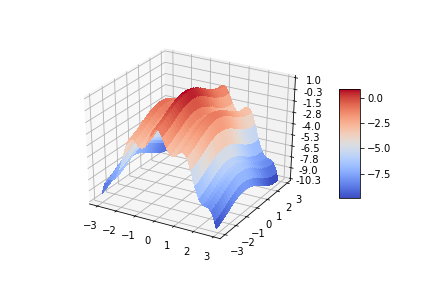
\includegraphics[width=100mm]{p7p_2d.png}
\caption{\label{fig3} Gráfica 3d.}
\end{figure}

\begin{figure}[H]
\centering
\begin{subfigure}[b]{0.40\linewidth}
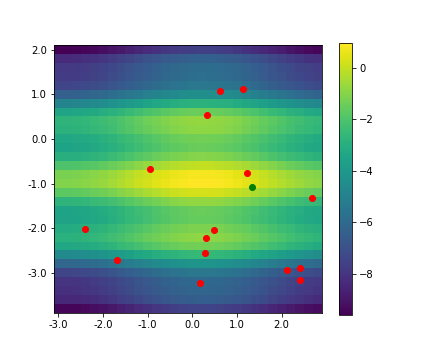
\includegraphics[width=\linewidth]{p7_v_t000.png}
\caption{Gráfica de posición inicial.}
\end{subfigure}
\begin{subfigure}[b]{0.40\linewidth}
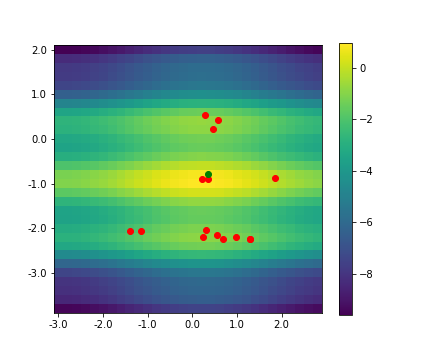
\includegraphics[width=\linewidth]{p7_v_t004.png}
\caption{Gráfica de posición en 4 pasos.}
\end{subfigure}
\caption{Gráfica que muestra la posición de los agentes}
\label{fig:westminster}
\end{figure}

\begin{figure}[H]
\centering
\begin{subfigure}[b]{0.40\linewidth}
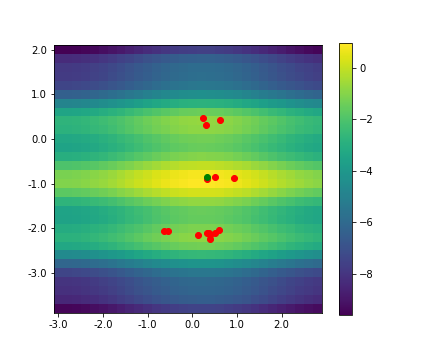
\includegraphics[width=\linewidth]{p7_v_t008.png}
\caption{Gráfica de posición en 8 pasos }
\end{subfigure}
\begin{subfigure}[b]{0.40\linewidth}
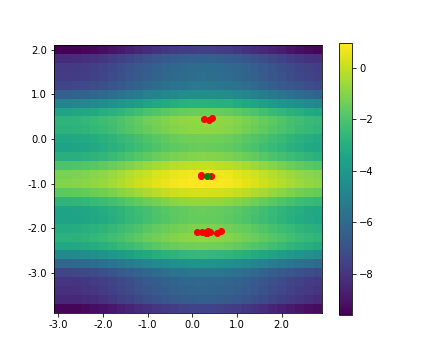
\includegraphics[width=\linewidth]{p7_v_t020.png}
\caption{Gráfica de posición en 20 pasos}
\end{subfigure}
\caption{Gráfica que muestra la posición de los agentes.}
\label{fig:westminster}
\end{figure}

\begin{figure}[H]
\centering
\begin{subfigure}[b]{0.40\linewidth}
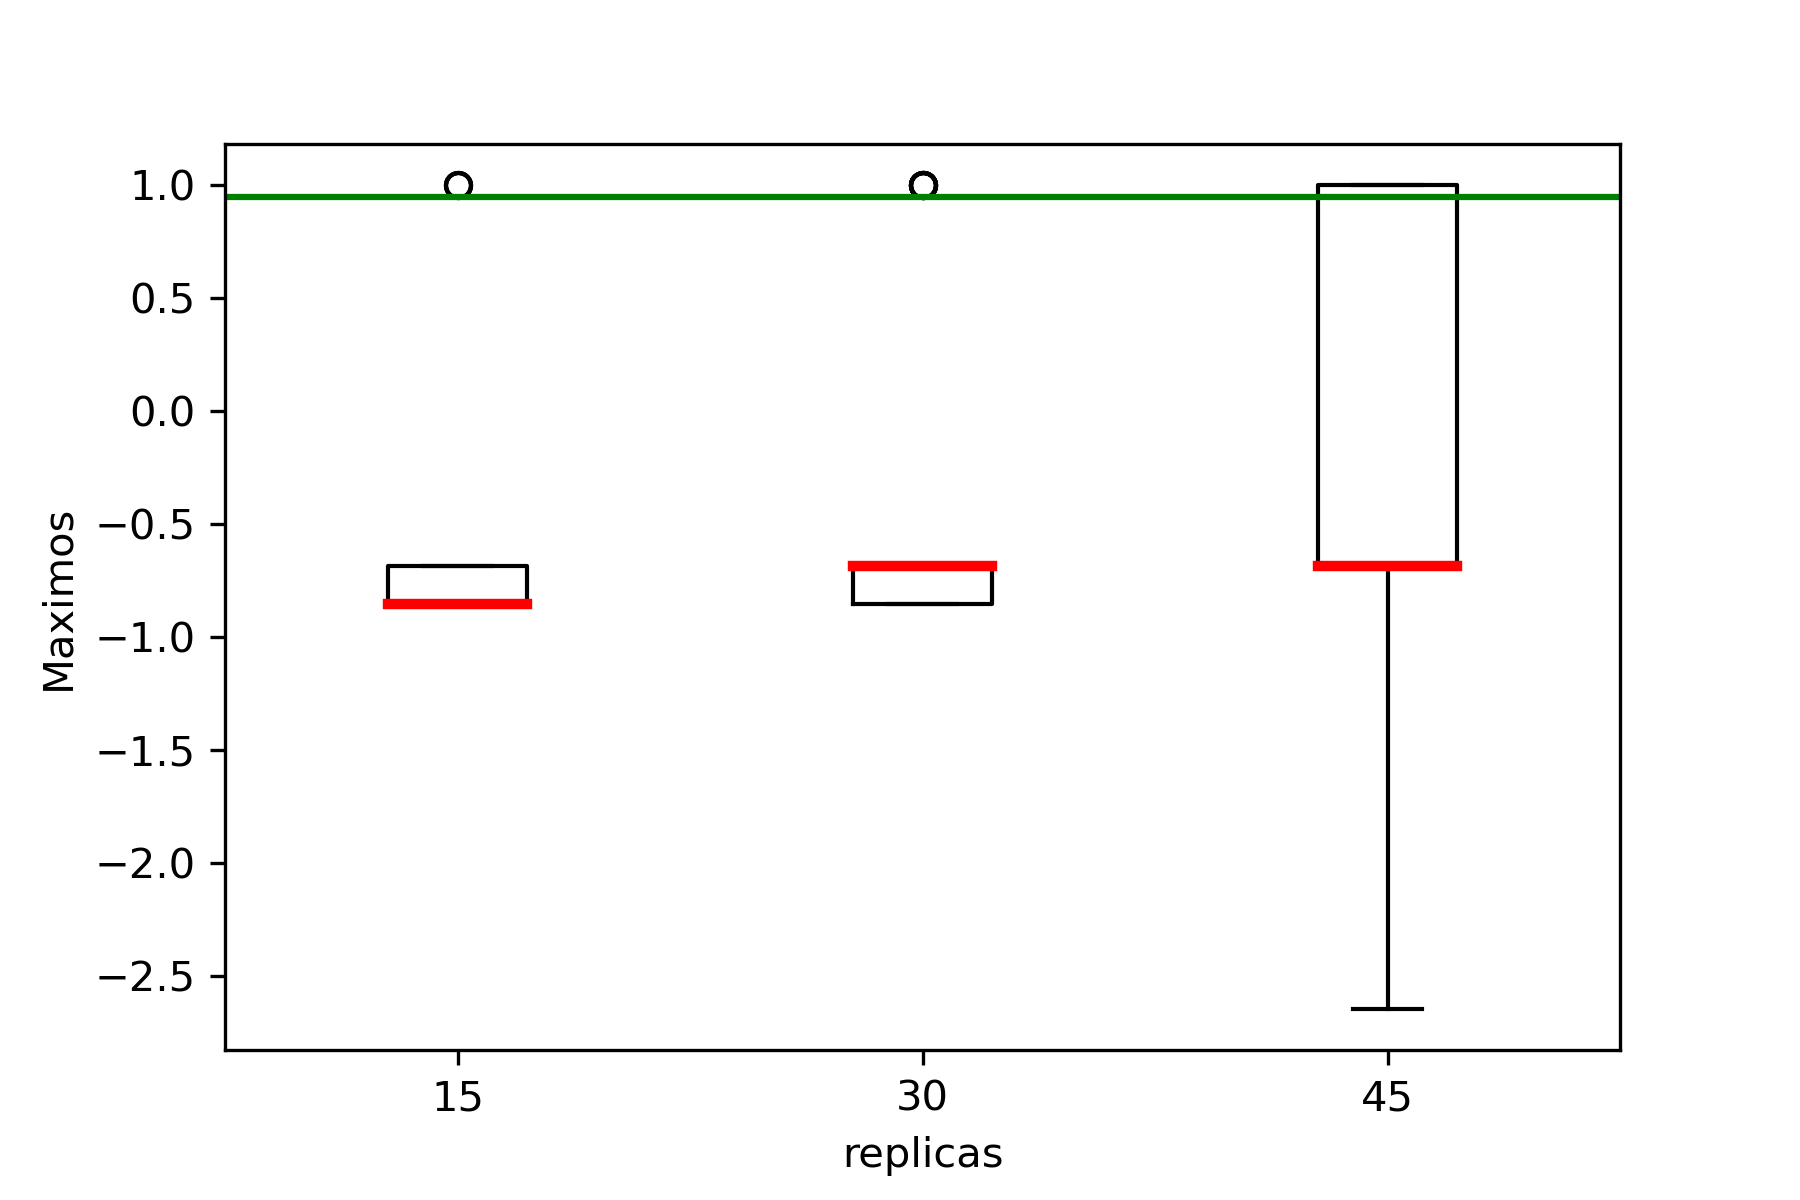
\includegraphics[width=\linewidth]{p7_p100.png}
\caption{100 pasos.}
\end{subfigure}
\begin{subfigure}[b]{0.40\linewidth}
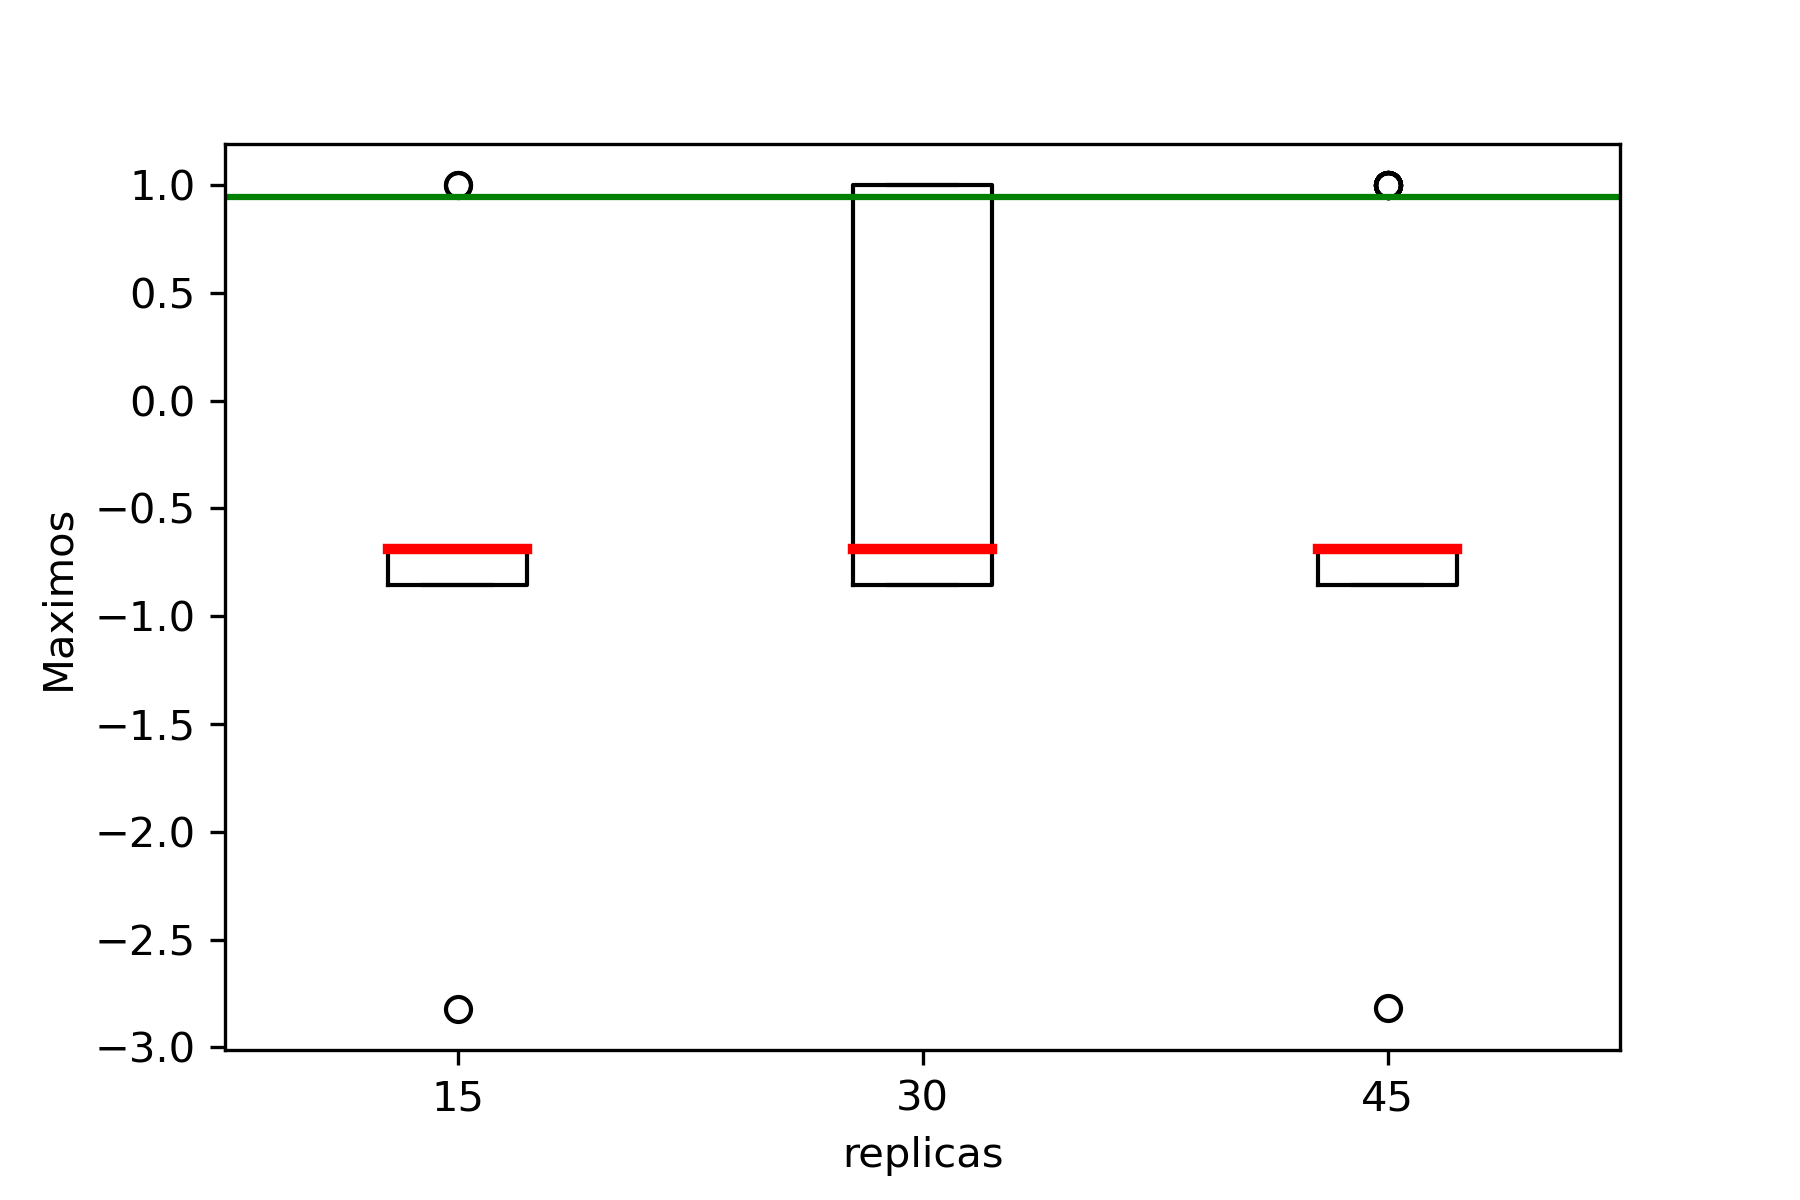
\includegraphics[width=\linewidth]{p7_p1000.png}
\caption{1000 pasos.}
\end{subfigure}
\caption{Gráfica caja bigote comparando replicas.}
\label{fig:westminster}
\end{figure}

\begin{figure}[H]
\centering
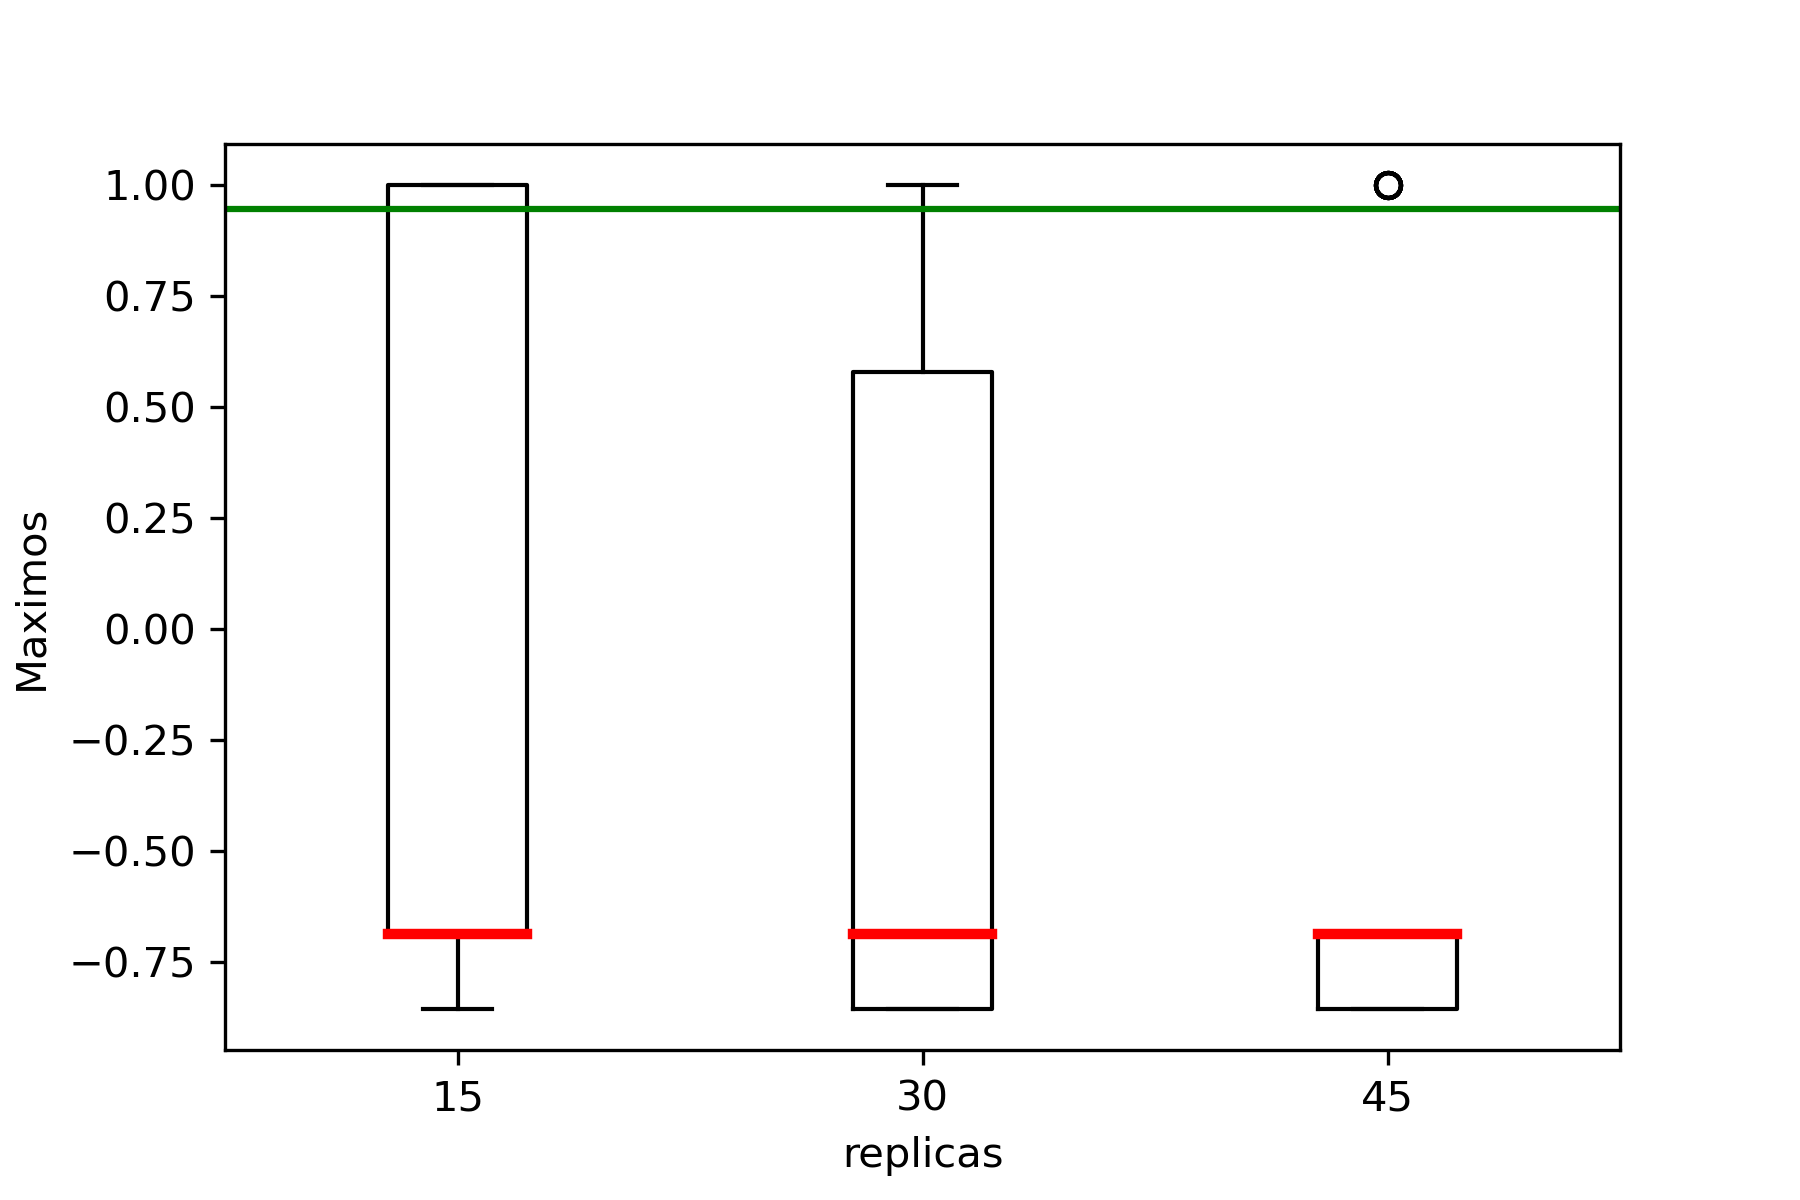
\includegraphics[width=80mm]{p7_p10000.png}
\caption{\label{fig3} Gráfica caja bigote comparando replicas en 10000 pasos.}
\end{figure}



\section{Reto 1}
El primer reto es cambiar la regla de movimiento de una solución $x$ (un vector de dimensión arbitraria) a la siguiente a la de recocido simulado, para optimizar una función {f(x)}, se genera para la solución actual $x$ un solo vecino $x' = x + \Delta x$ (algún desplazamiento local). Se calcula $ \delta = f(X') - f(x)$ (para minimizar; maximizando la resta se hace al revés). Si $\delta > 0$, siempre se acepta el vecino $x'$ como la solución actual ya que representa una mejora. Si  $\delta < 0$ se acepta a $x'$ con probabilidad $exp(\delta / T )$ y rechaza en otro caso. Aqui $T$ es una temperatura que decrece en aquellos pasos donde se acepta una empeora; la reducción se logra multiplicando el valor actual de $T$ con $\xi < 1$, como por ejemplo 0.995 \cite{Satu_Elisa_Schaeffer}.

A continuación se muestra una parte del código, donde se realiza el movimiento de los agentes, el código completo se encuentra en GitHub \cite{Denisse_Leyva}, además de los gif que muestran el movimiento de los agentes. 

\renewcommand{\listingscaption}{Código}
\begin{listing}[H]
  \begin{minted}[linenos,mathescape,texcl]{clojure}
r = agentes.iloc[i]
xp = r.x + r.dx
yp = r.y + r.dy

if  xp < low+step:
    xp = r.x
elif xp > high-step:
    xp = r.x
if  yp < low+step:
    yp = r.y
elif yp > high-step:
    yp = r.y

delta = g(xp, yp) - g(r.x, r.y)
prob = exp(delta/r.t)
if delta > 0:
    agentes.at[i, 'x'] = xp
    agentes.at[i, 'y'] = yp
else:
    if random() < (prob):
        agentes.at[i, 'x'] = xp
        agentes.at[i, 'y'] = yp
        agentes.at[i, 't'] = r.t * xi
mejor = g(r.x, r.y)
if mejor > best:
    best = g(r.x, r.y)
    bestx = r.x
    besty = r.y
if mejor > r.best:
    agentes.at[i, 'best'] = mejor
  
    \end{minted}
  \label{lst:fibo}
  \caption{Realiza el movimiento de los agentes con la regla del recocido simulado.}
\end{listing}

\begin{figure}[H]
\centering
\begin{subfigure}[b]{0.40\linewidth}
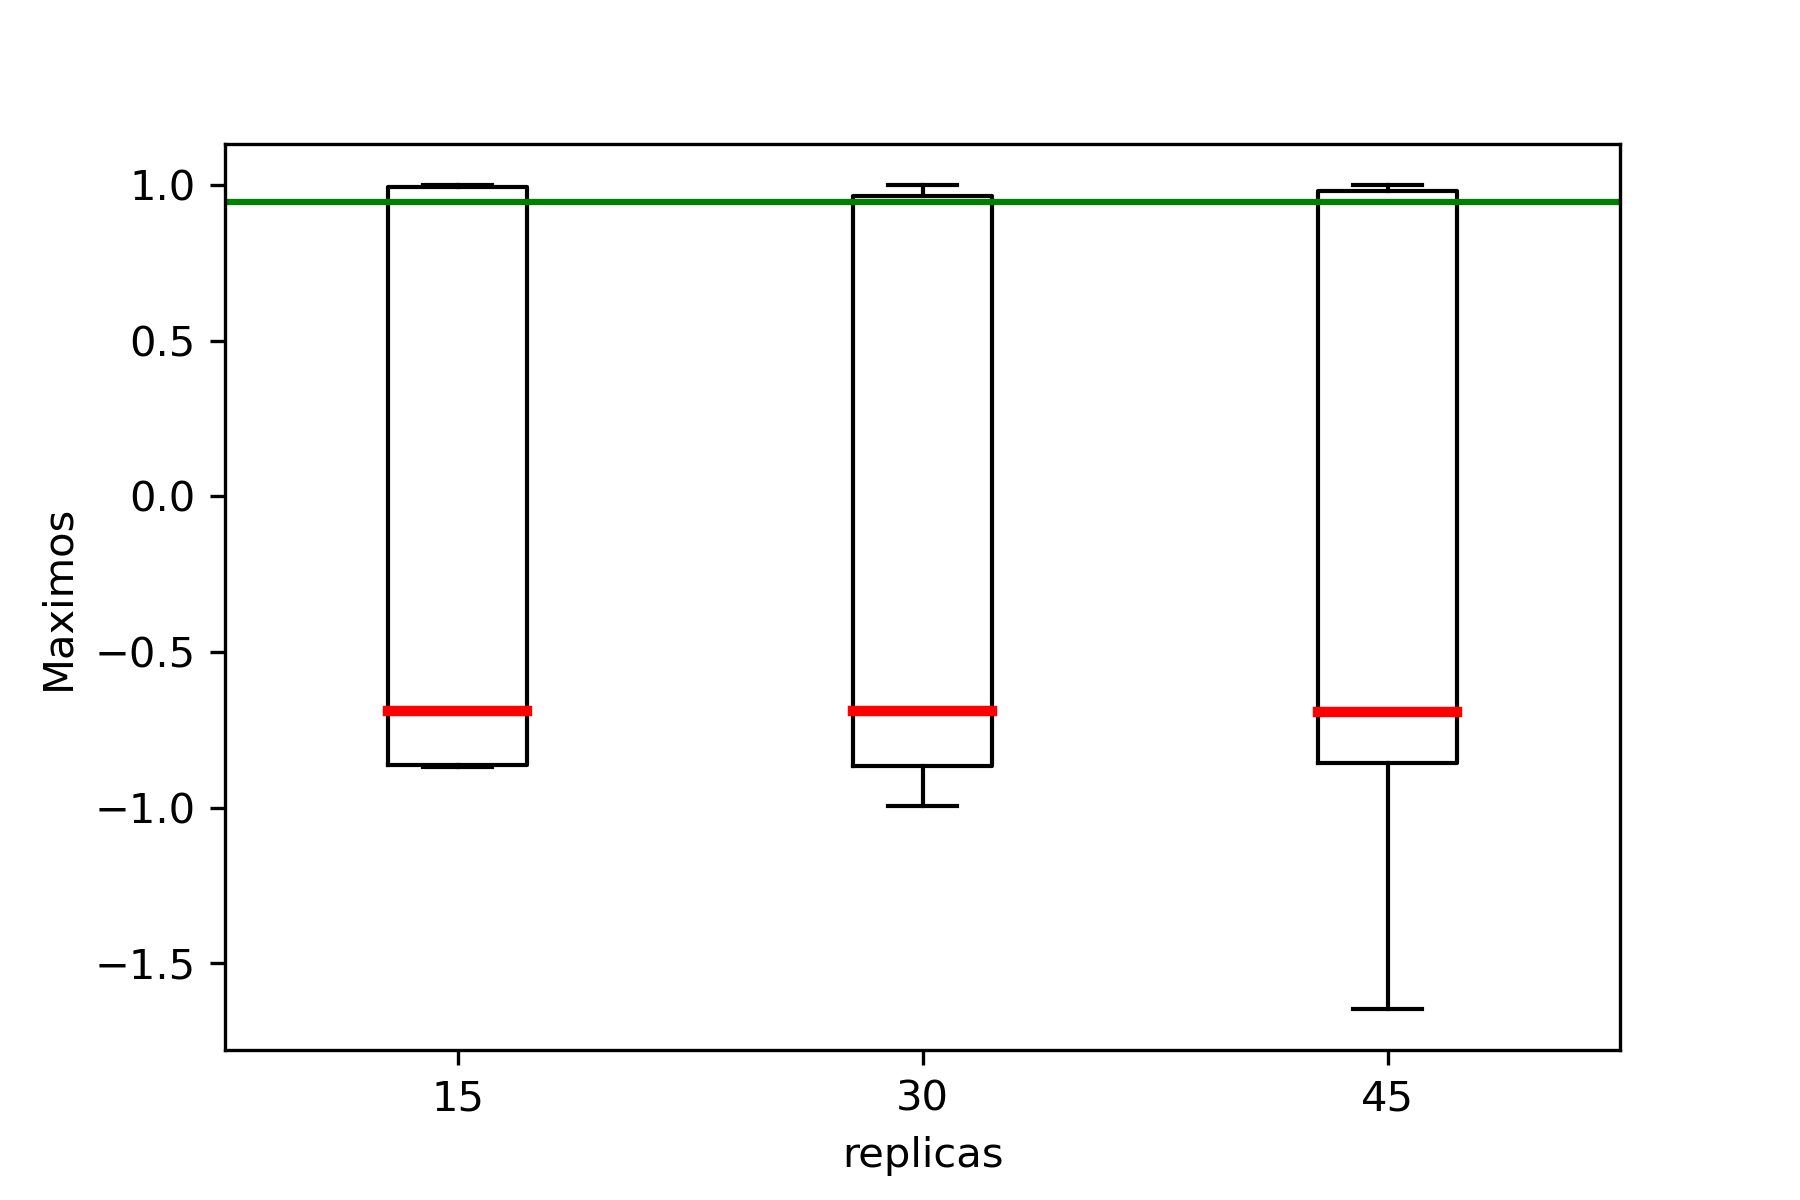
\includegraphics[width=\linewidth]{p7_p100_T10_xi33.png}
\caption{Temperatura 10 con $\xi$ 0.33 }
\end{subfigure}
\begin{subfigure}[b]{0.40\linewidth}
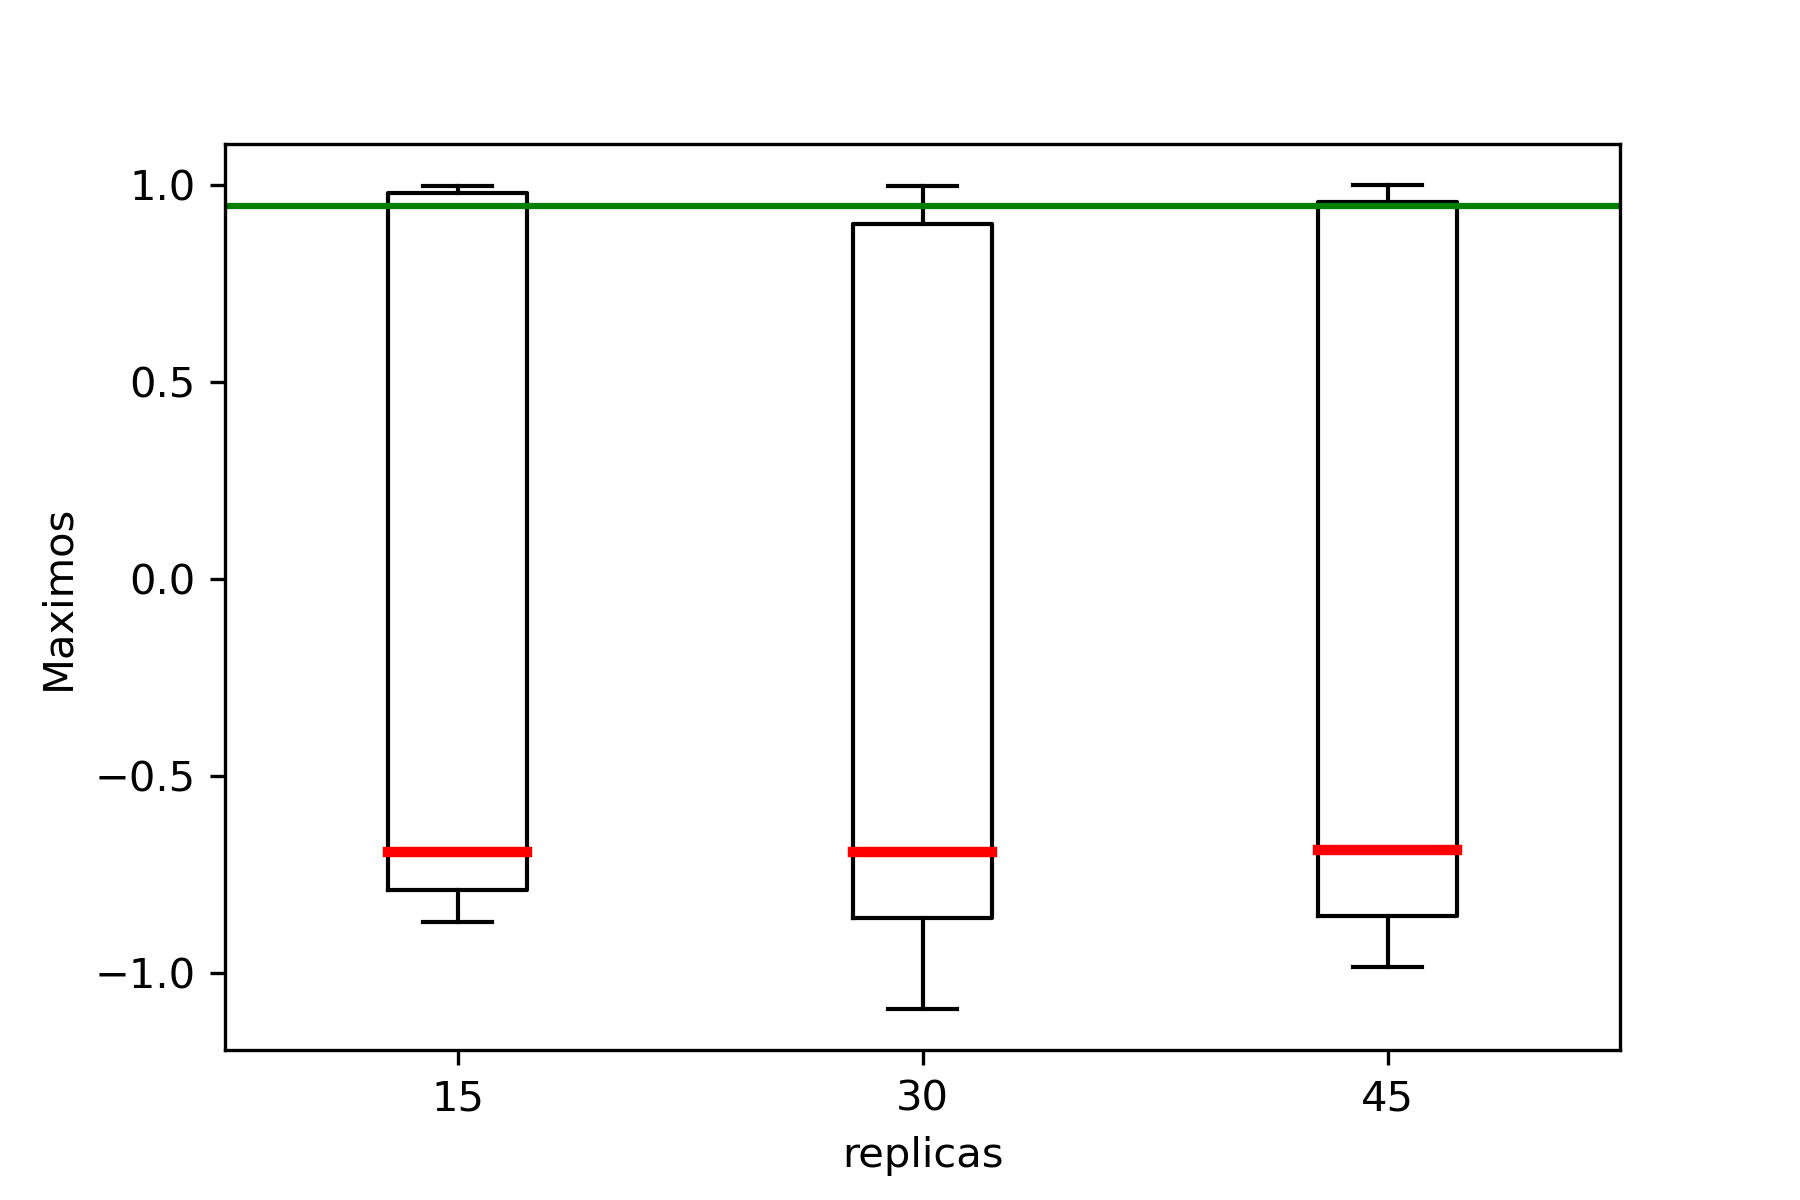
\includegraphics[width=\linewidth]{p7_p100_T10_xi66.png}
\caption{Temperatura 10 con $\xi$ 0.66}
\end{subfigure}
\caption{Gráfica caja bigote de 100 pasos en función a temperatura y $\xi$.}
\label{fig:westminster}
\end{figure}

\begin{figure}[H]
\centering
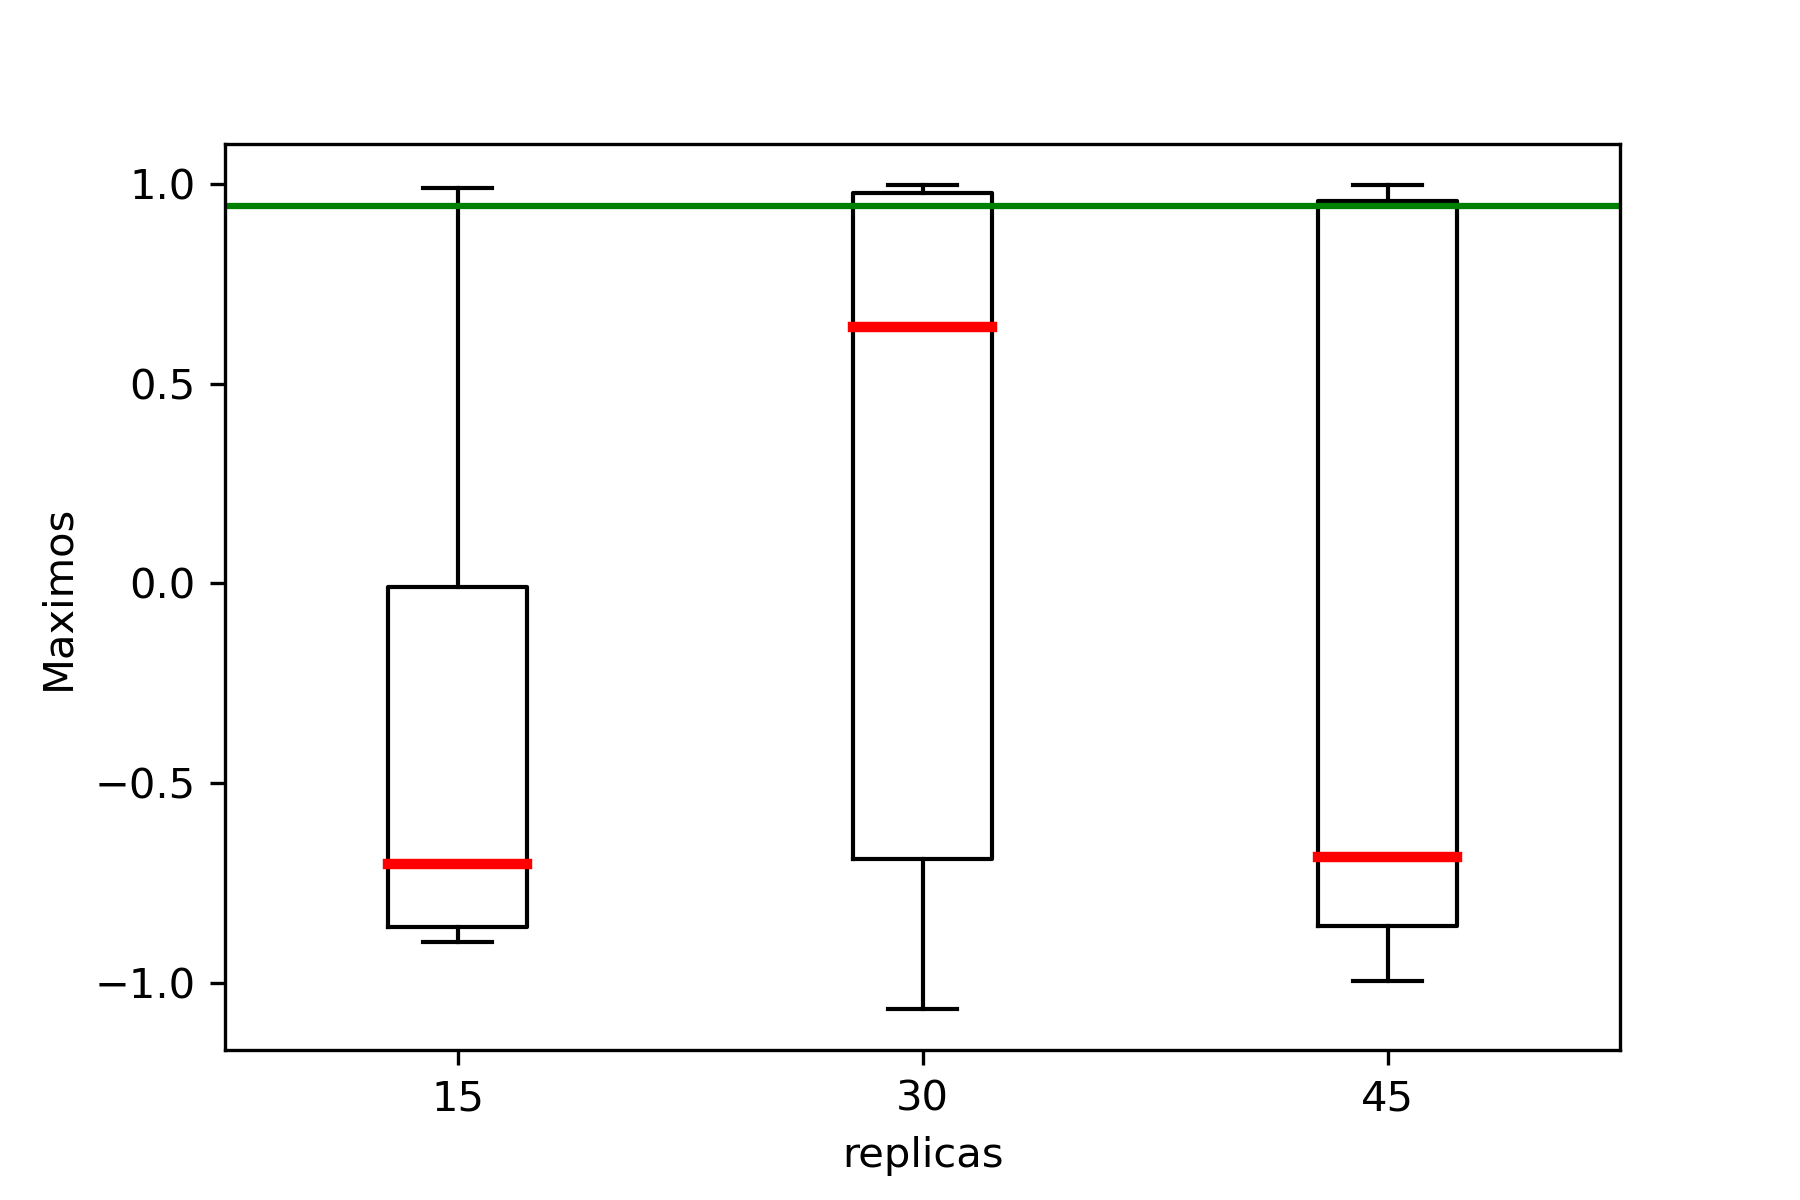
\includegraphics[width=80mm]{p7_p100_T10_xi99.png}
\caption{\label{fig3} Gráfica caja bigote de 100 pasos en función a temperatura=10 y $\xi$=0.99.}
\end{figure}

\begin{figure}[H]
\centering
\begin{subfigure}[b]{0.40\linewidth}
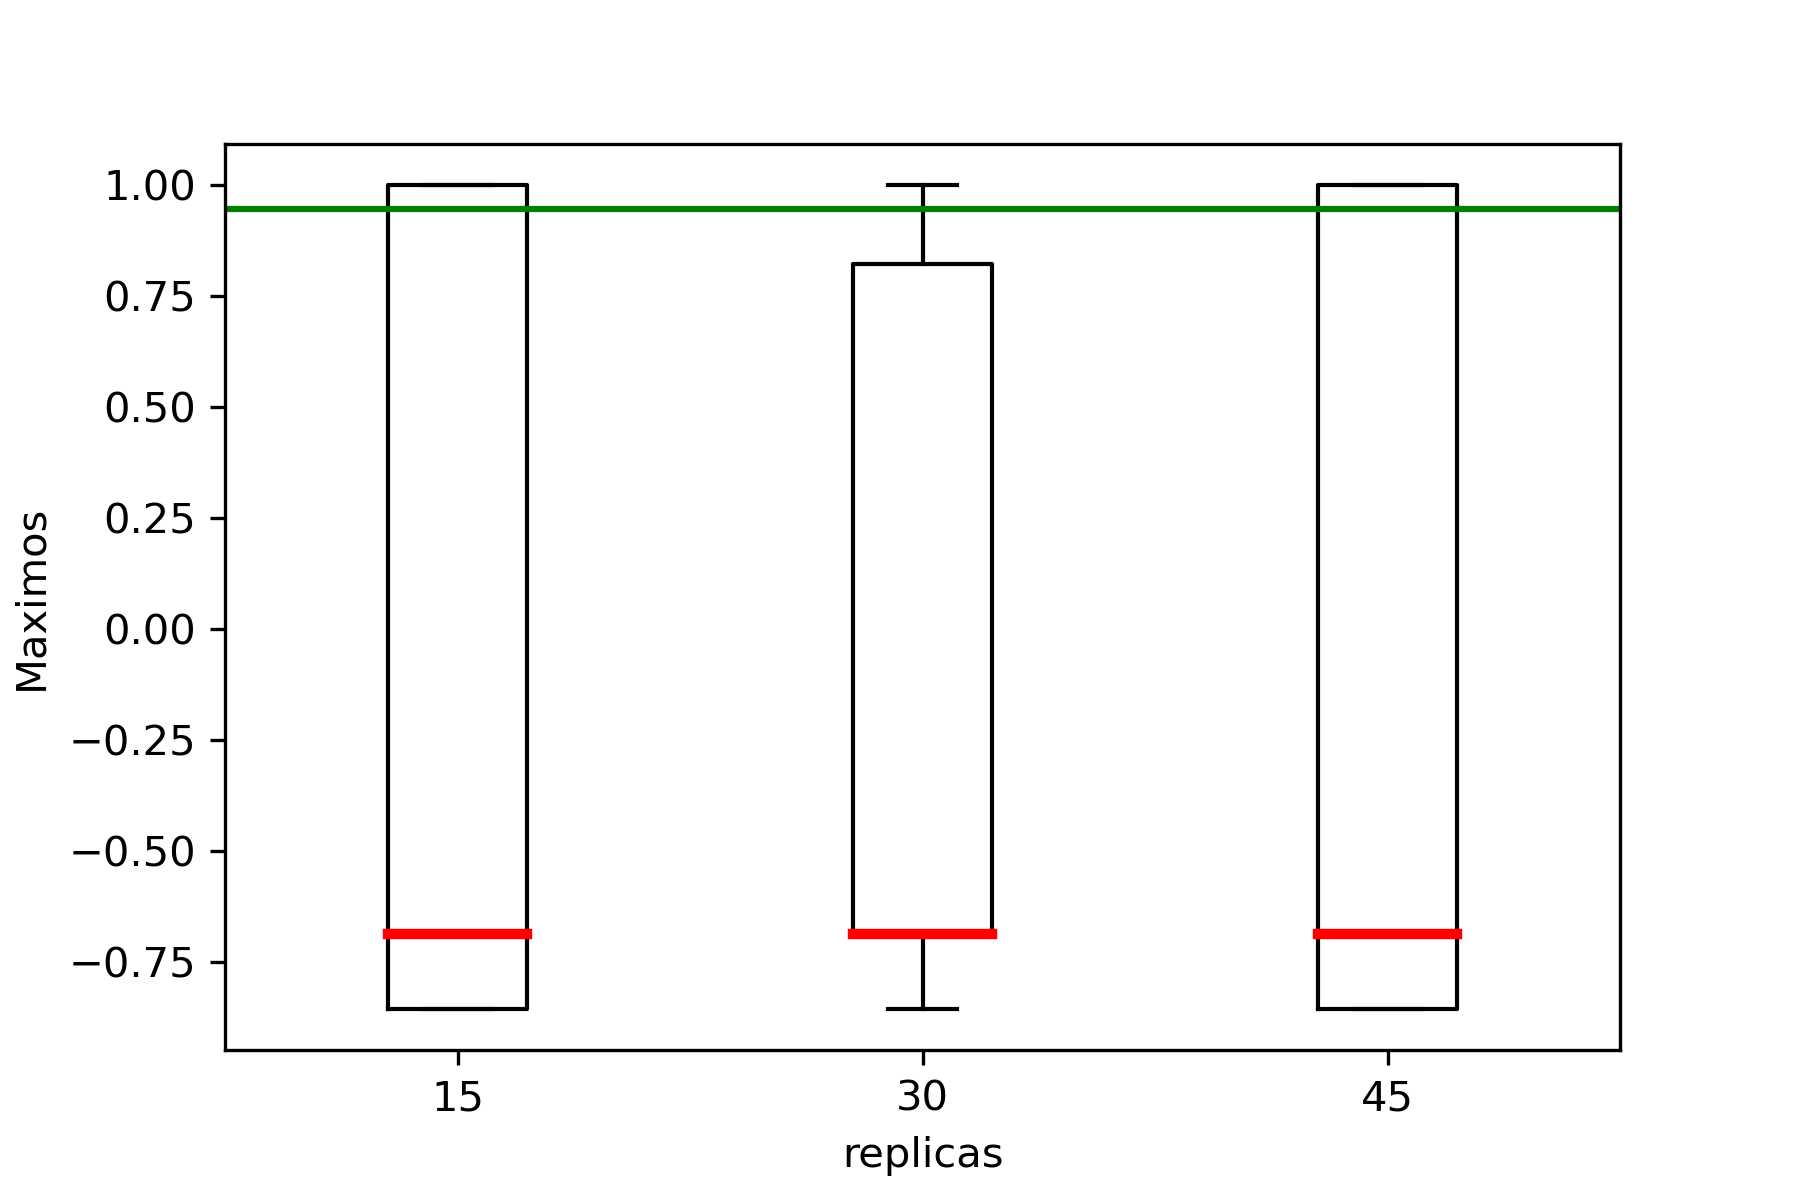
\includegraphics[width=\linewidth]{p7_p10000_T100_xi33.png}
\caption{Temperatura 100 con $\xi$ 0.33.}
\end{subfigure}
\begin{subfigure}[b]{0.40\linewidth}
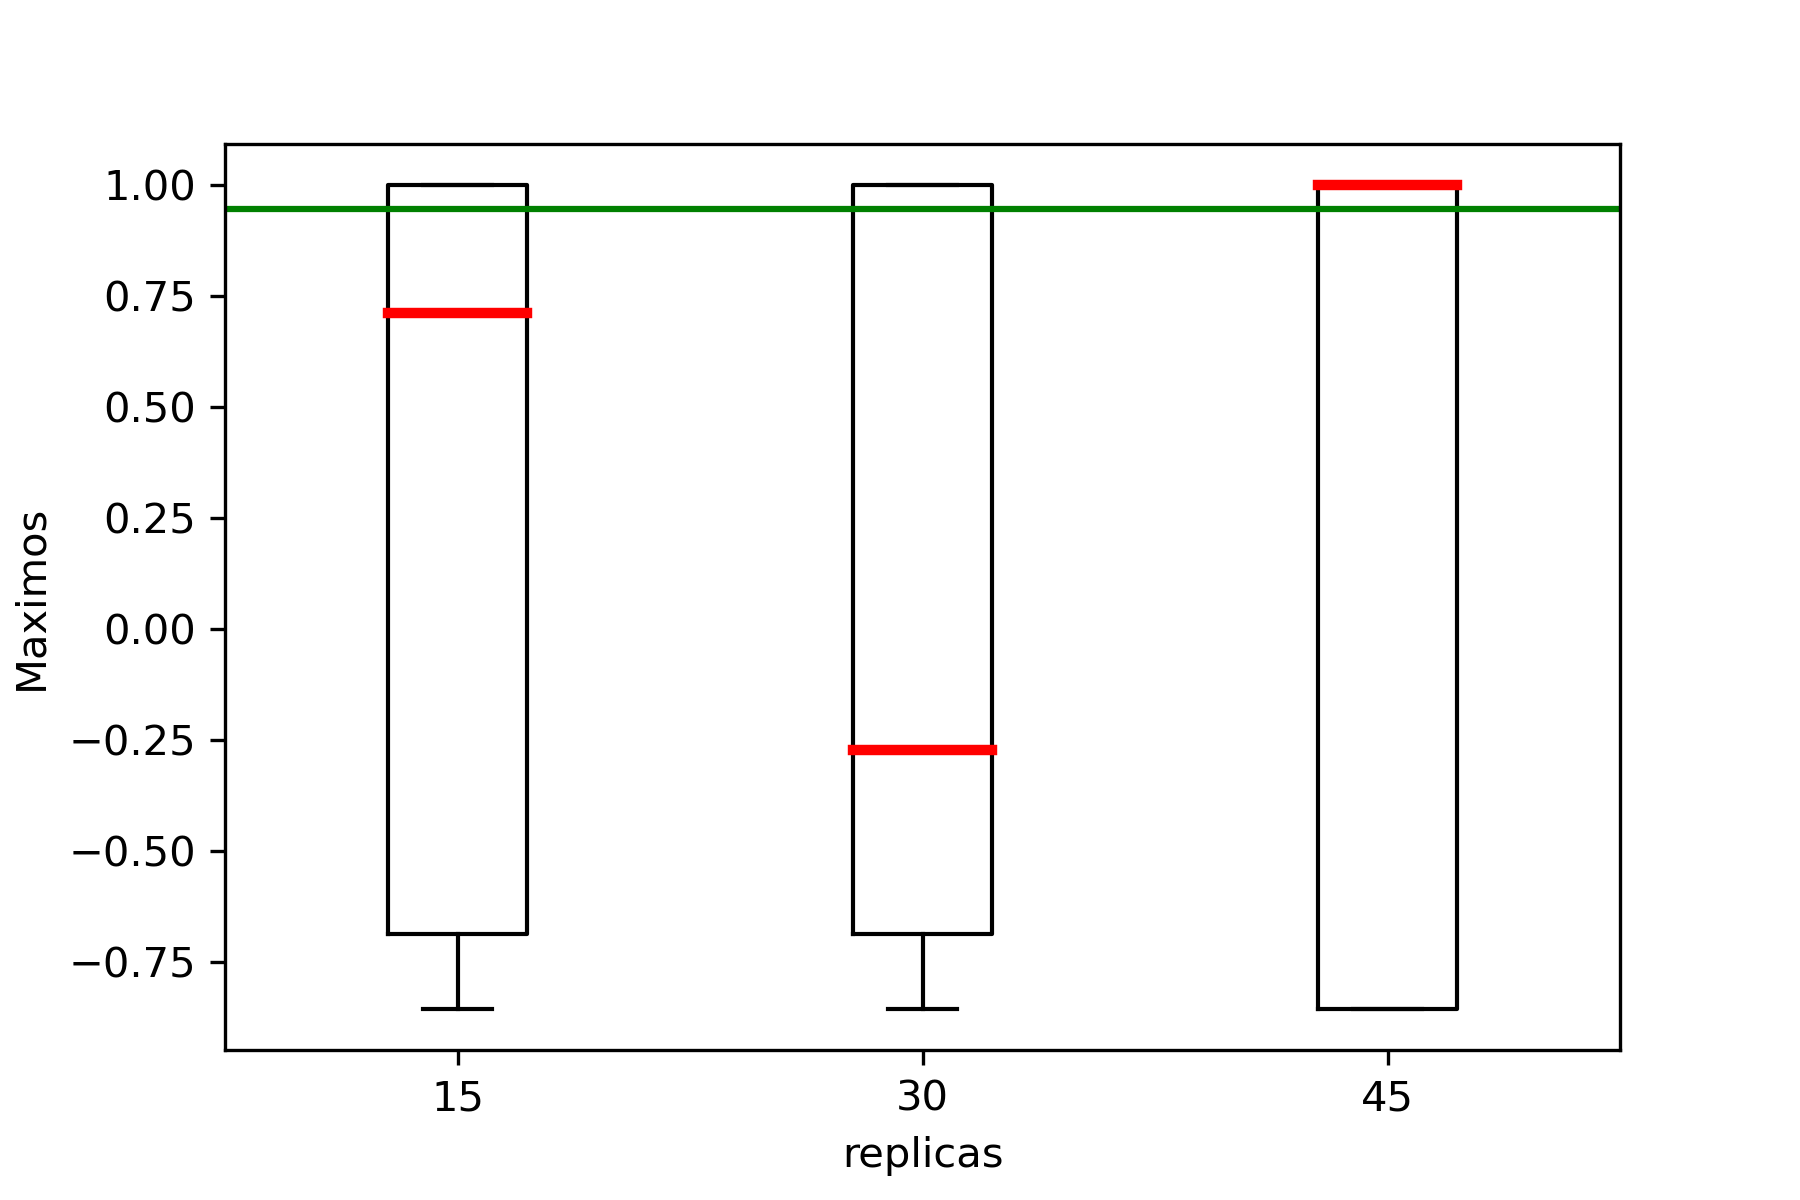
\includegraphics[width=\linewidth]{p7_p10000_T100_xi66.png}
\caption{Temperatura 100 con $\xi$ 0.66.}
\end{subfigure}
\caption{Gráfica caja bigote de 10000 pasos en función a temperatura y $\xi$.}
\label{fig:westminster}
\end{figure}

\begin{figure}[H]
\centering
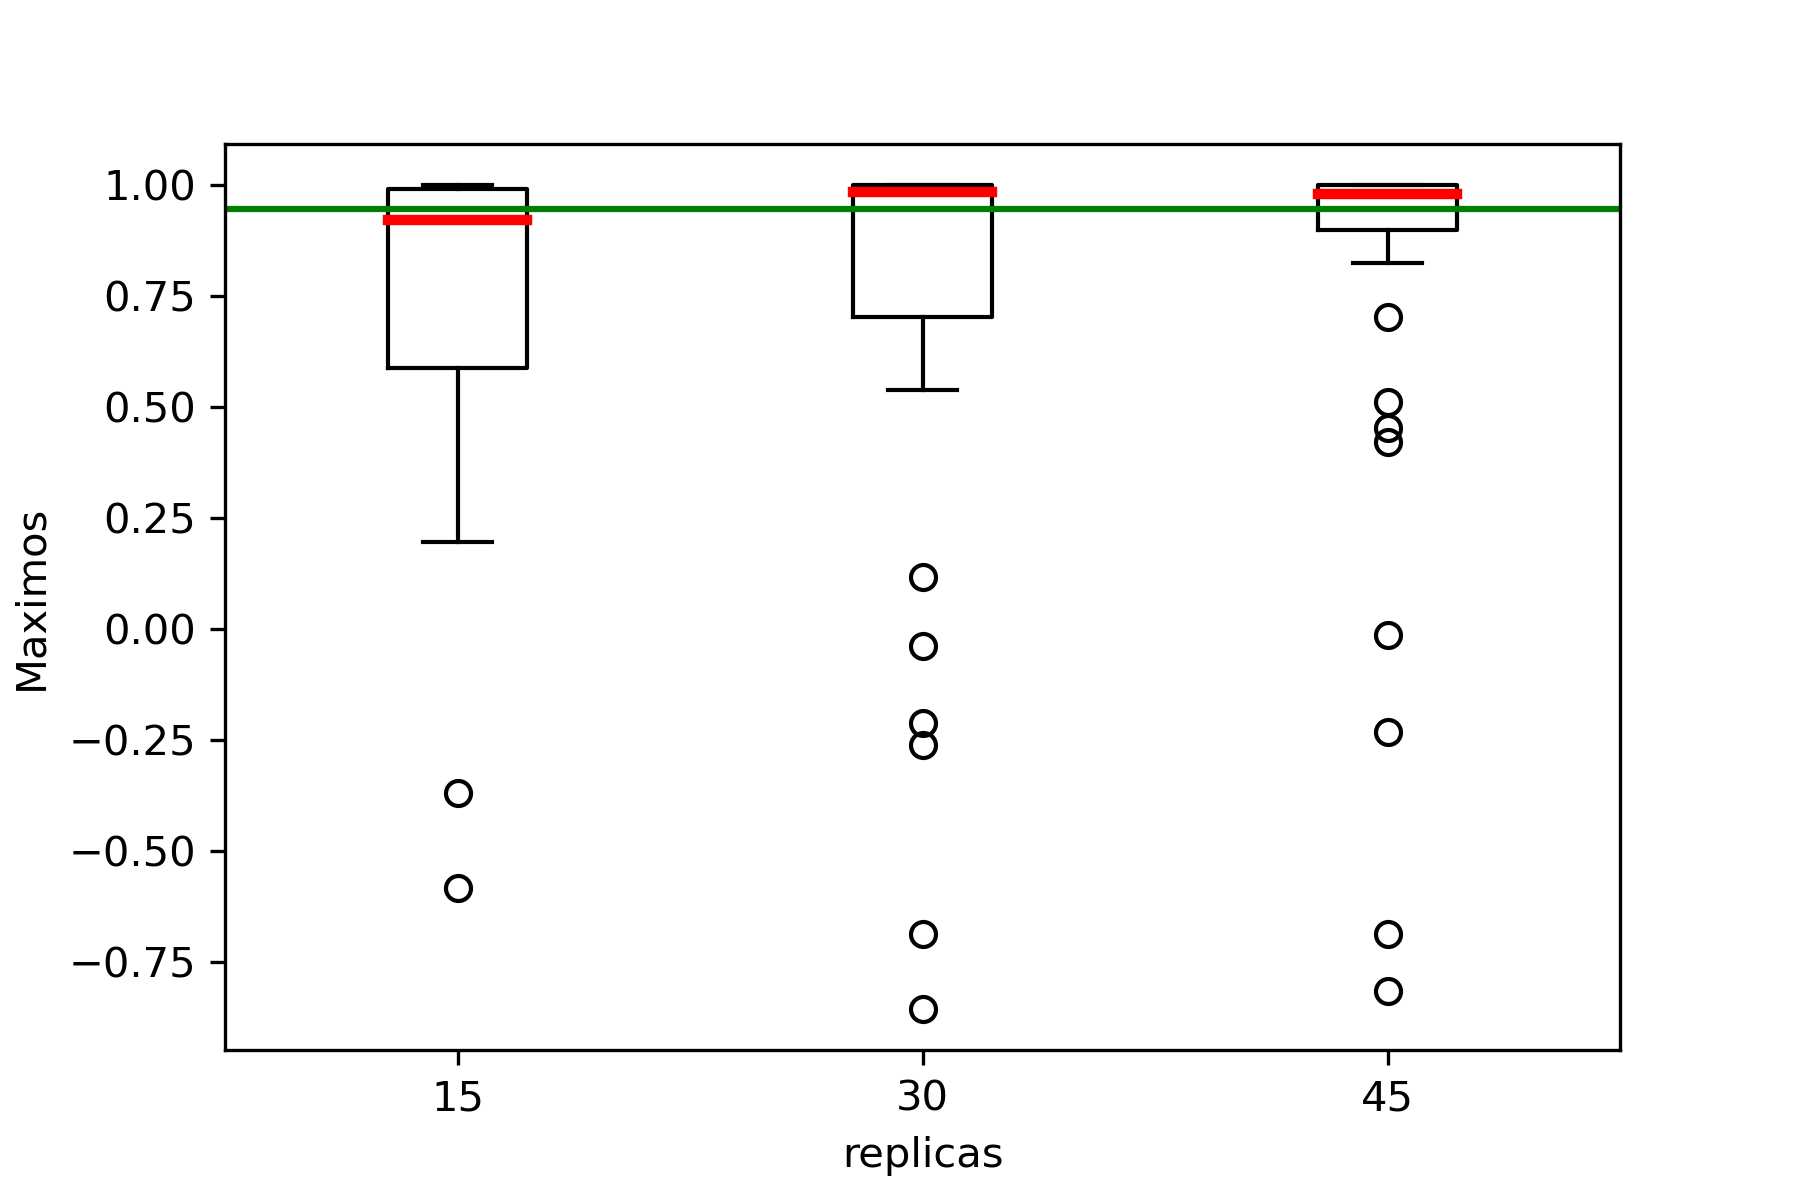
\includegraphics[width=80mm]{p7_p10000_T100_xi99.png}
\caption{\label{fig3} Gráfica caja bigote de 10000 pasos en función a temperatura=100 y $\xi$=0.99.}
\end{figure}


\section{Reto 2}
El segundo reto es comparar sí o no hay diferencia estadísticamente significativa entre el método de la tarea base y el método del primer reto en términos de la precisión del resultado obtenido (es decir, la diferencia entre el resultado reportado y el óptimo global) en función del número de iteraciones y el número de réplicas \cite{Satu_Elisa_Schaeffer}.

Al observar las siguientes gráficas podemos concluir que es mejor el metodo recocido simulado ya que entre mayor sea la temperatura y mayor sea $\xi$ el resultado del promedio de las muestras esta mucho más cerca en el valor deseado.

\begin{figure}[H]
\centering
\begin{subfigure}[b]{0.40\linewidth}
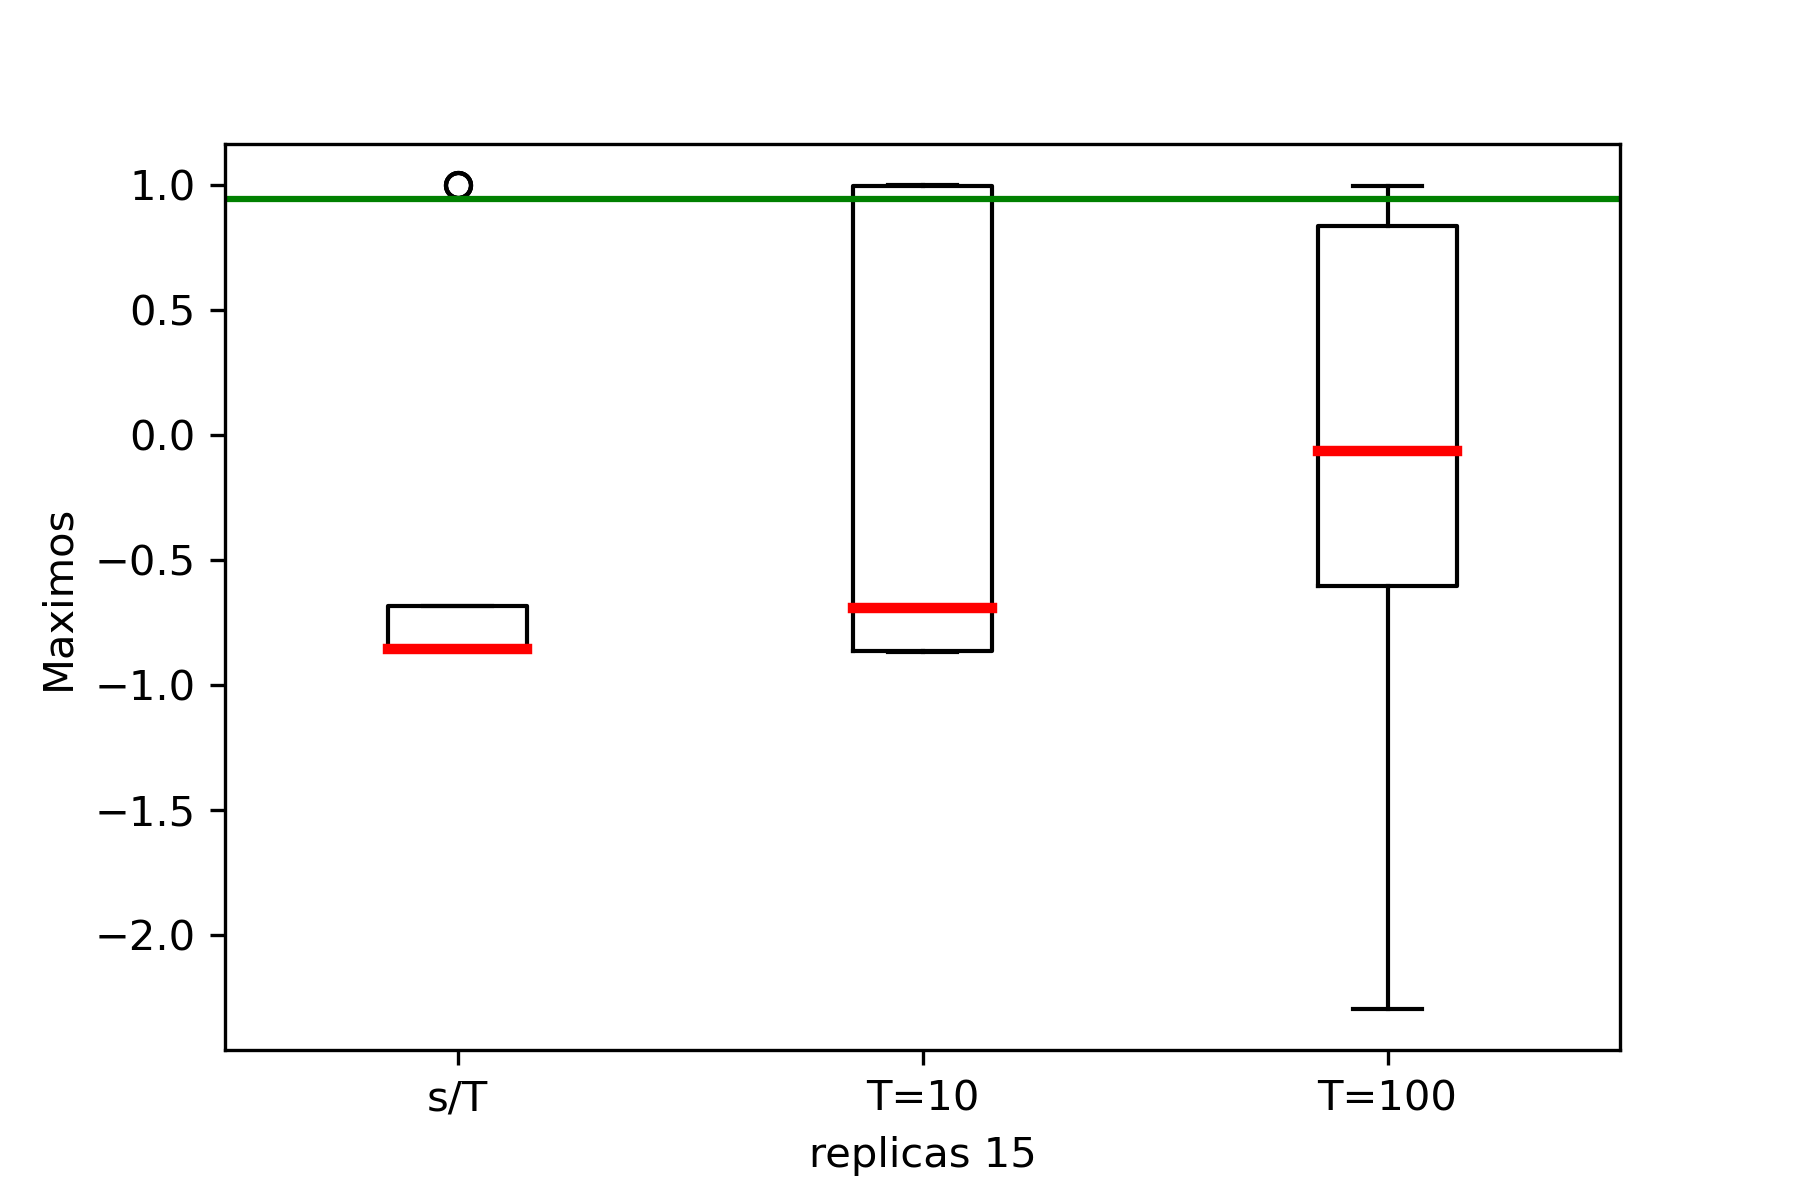
\includegraphics[width=\linewidth]{p7_p100_r15.png}
\caption{100 pasos.}
\end{subfigure}
\begin{subfigure}[b]{0.40\linewidth}
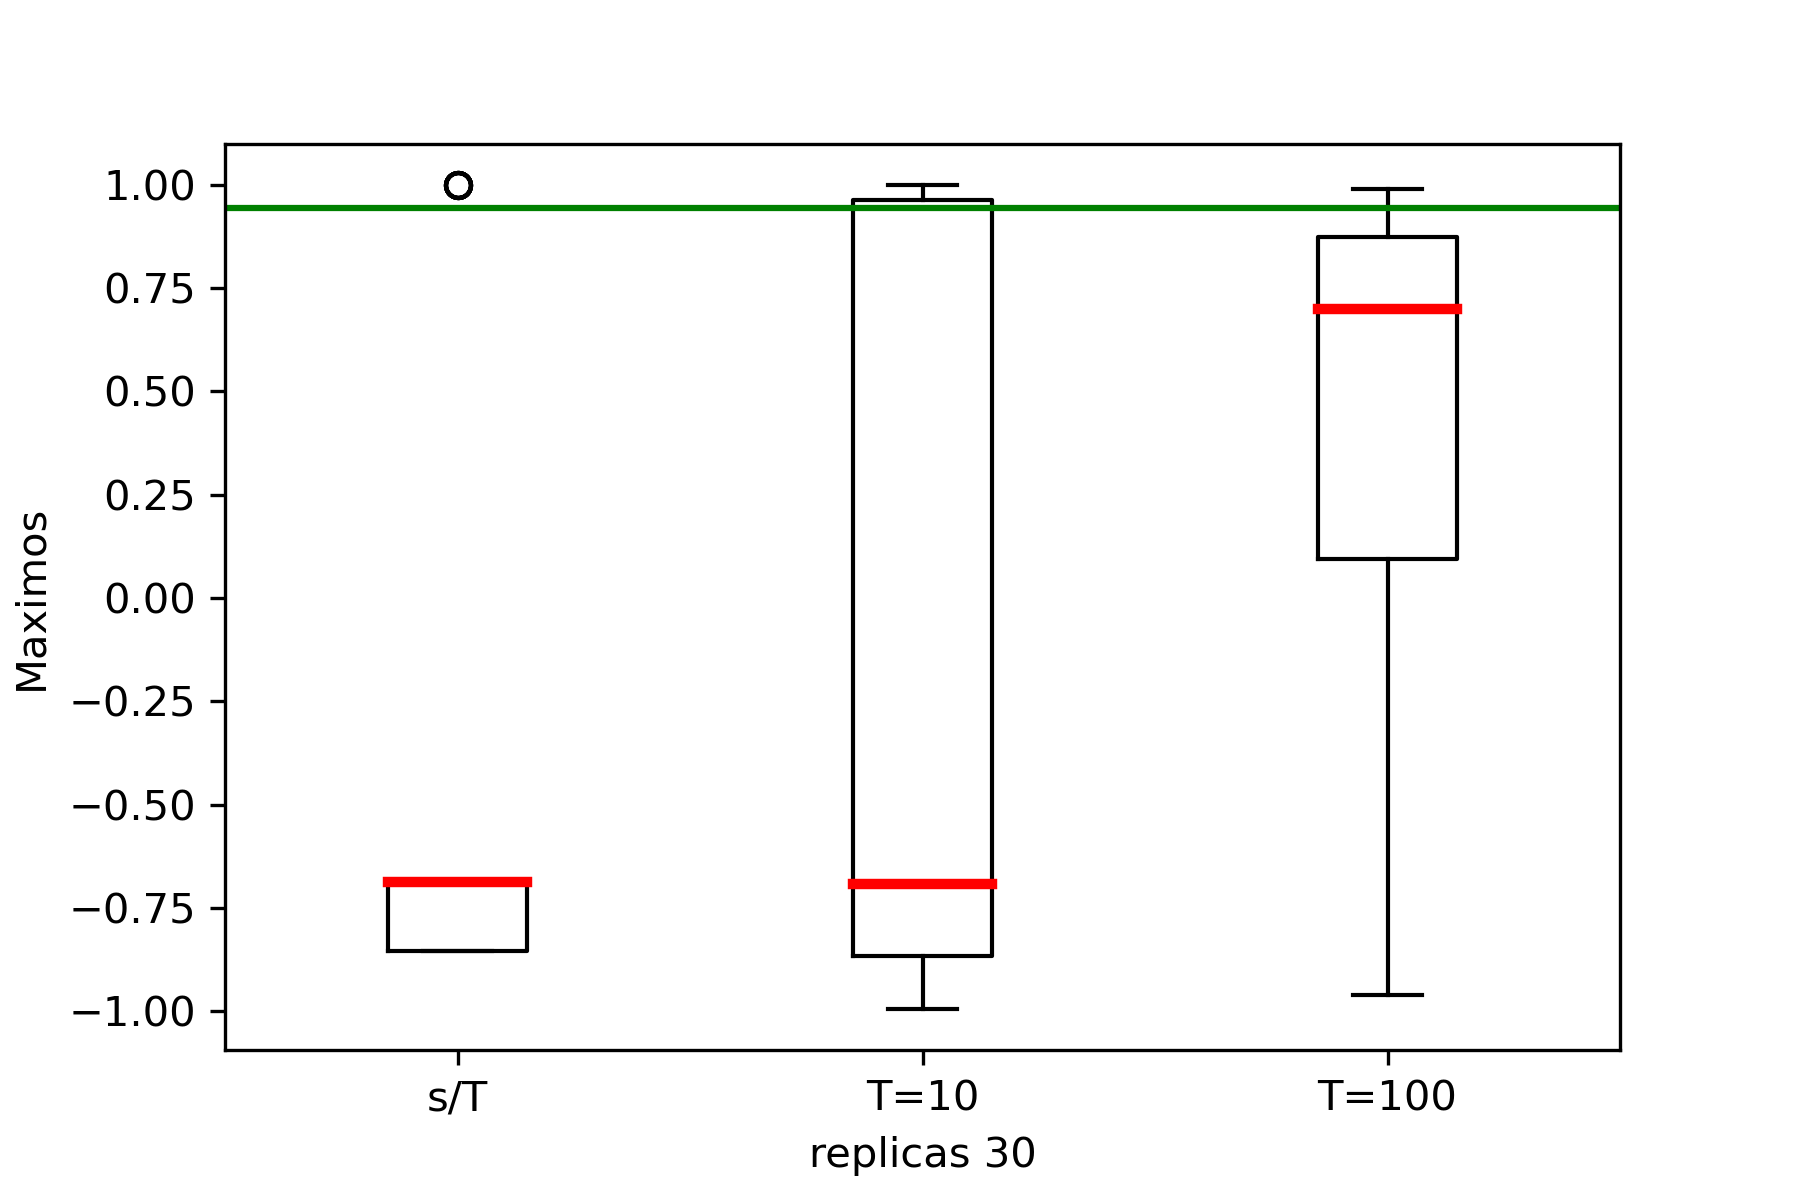
\includegraphics[width=\linewidth]{p7_p100_r30.png}
\caption{100 pasos.}
\end{subfigure}
\caption{Gráfica caja bigote de pasos comparando muestras sin y con temperatura y $\xi$.}
\label{fig:westminster}
\end{figure}

\begin{figure}[H]
\centering
\begin{subfigure}[b]{0.40\linewidth}
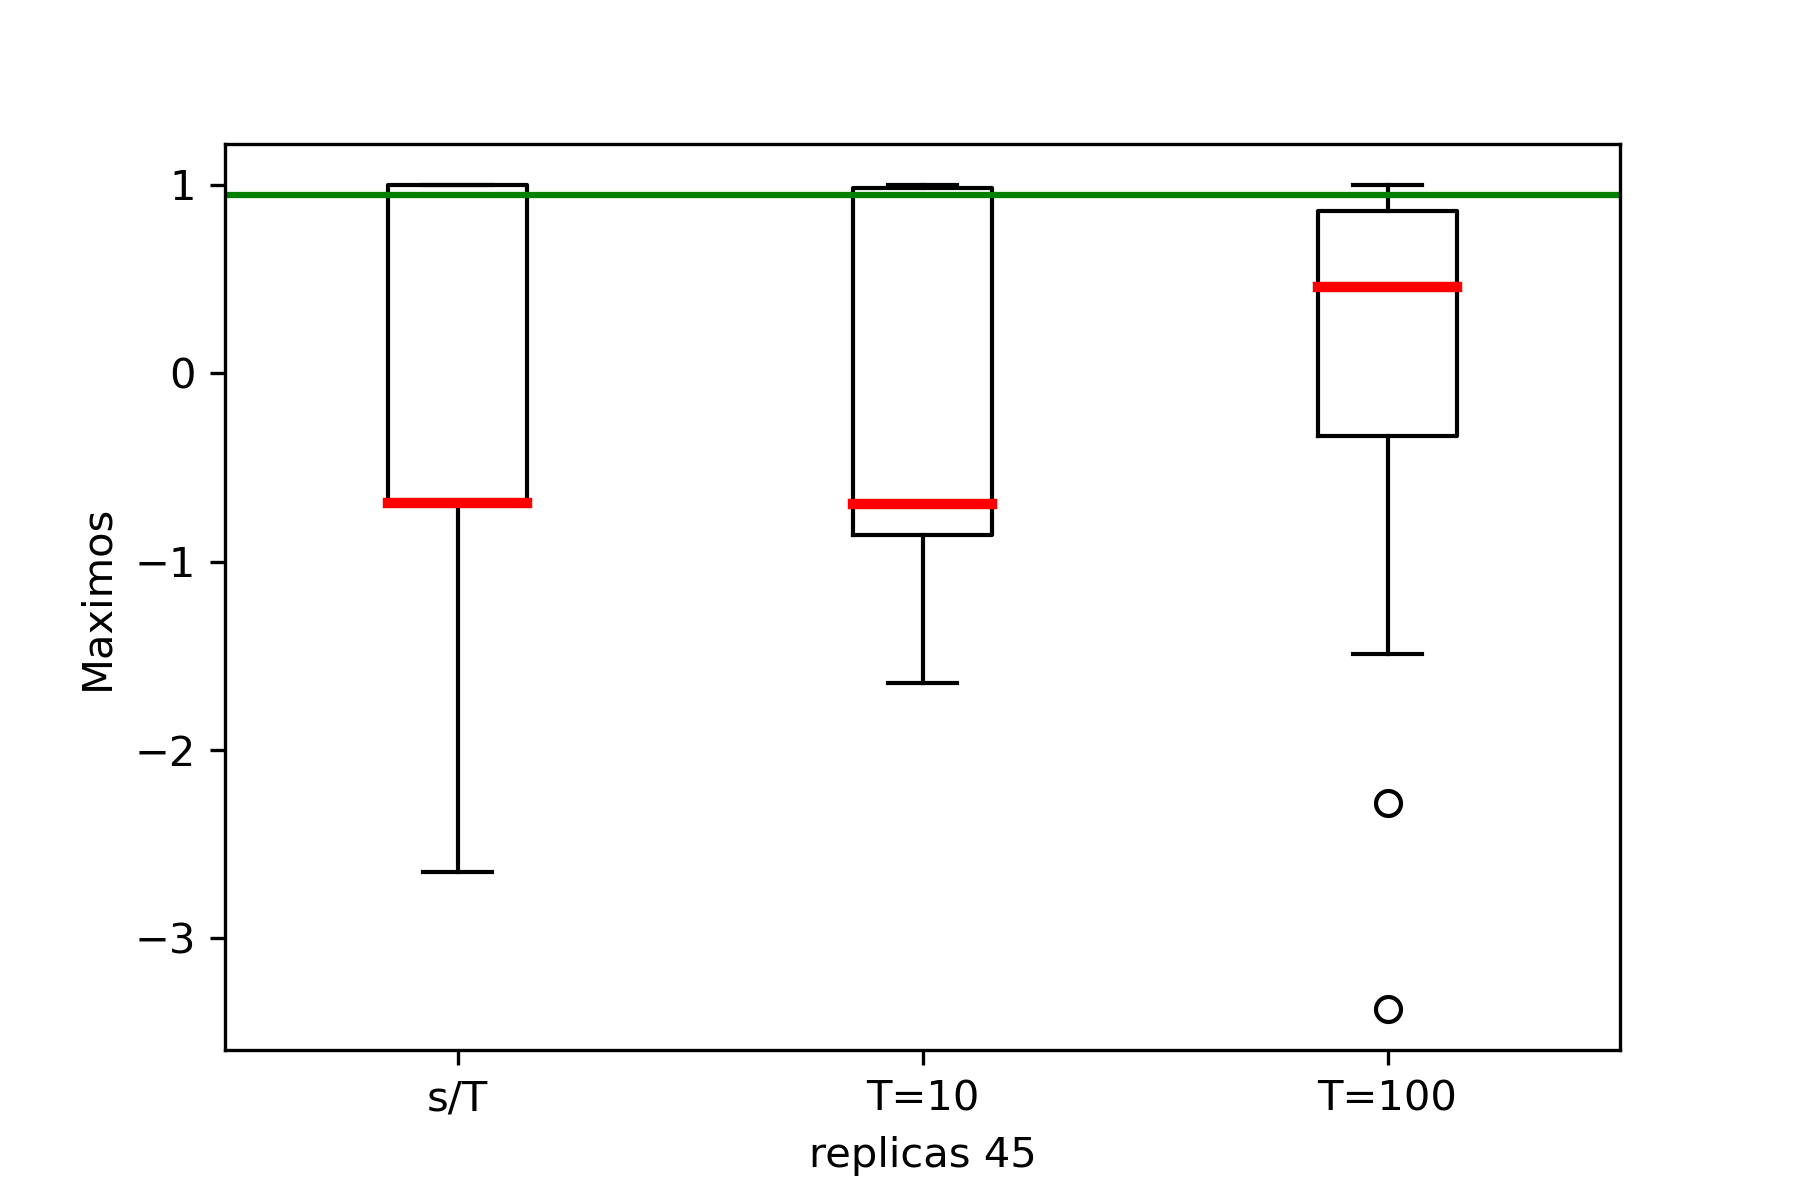
\includegraphics[width=\linewidth]{p7_p100_r45.png}
\caption{100 pasos.}
\end{subfigure}
\begin{subfigure}[b]{0.40\linewidth}
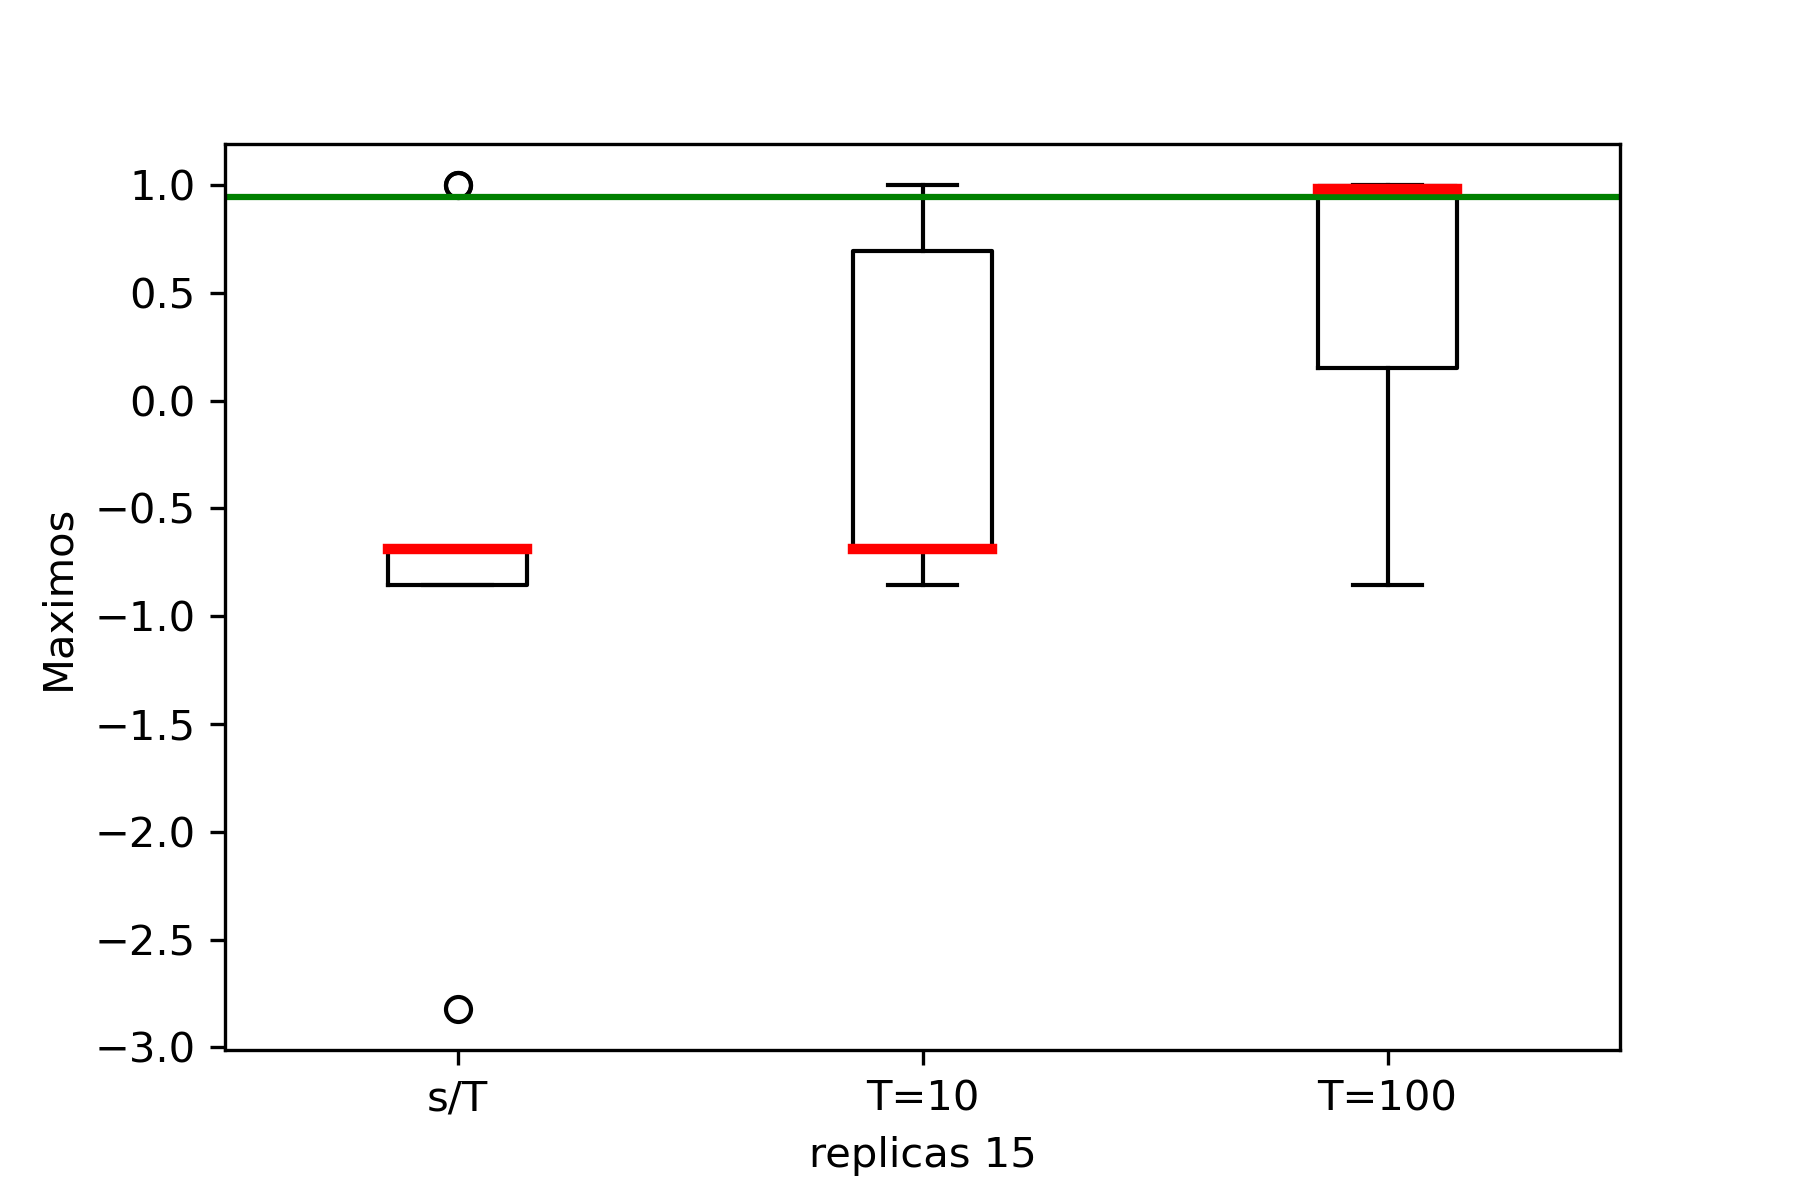
\includegraphics[width=\linewidth]{p7_p1000_r15.png}
\caption{1000 pasos.}
\end{subfigure}
\caption{Gráfica caja bigote de pasos comparando muestras sin y con temperatura y $\xi$.}
\label{fig:westminster}
\end{figure}

\begin{figure}[H]
\centering
\begin{subfigure}[b]{0.40\linewidth}
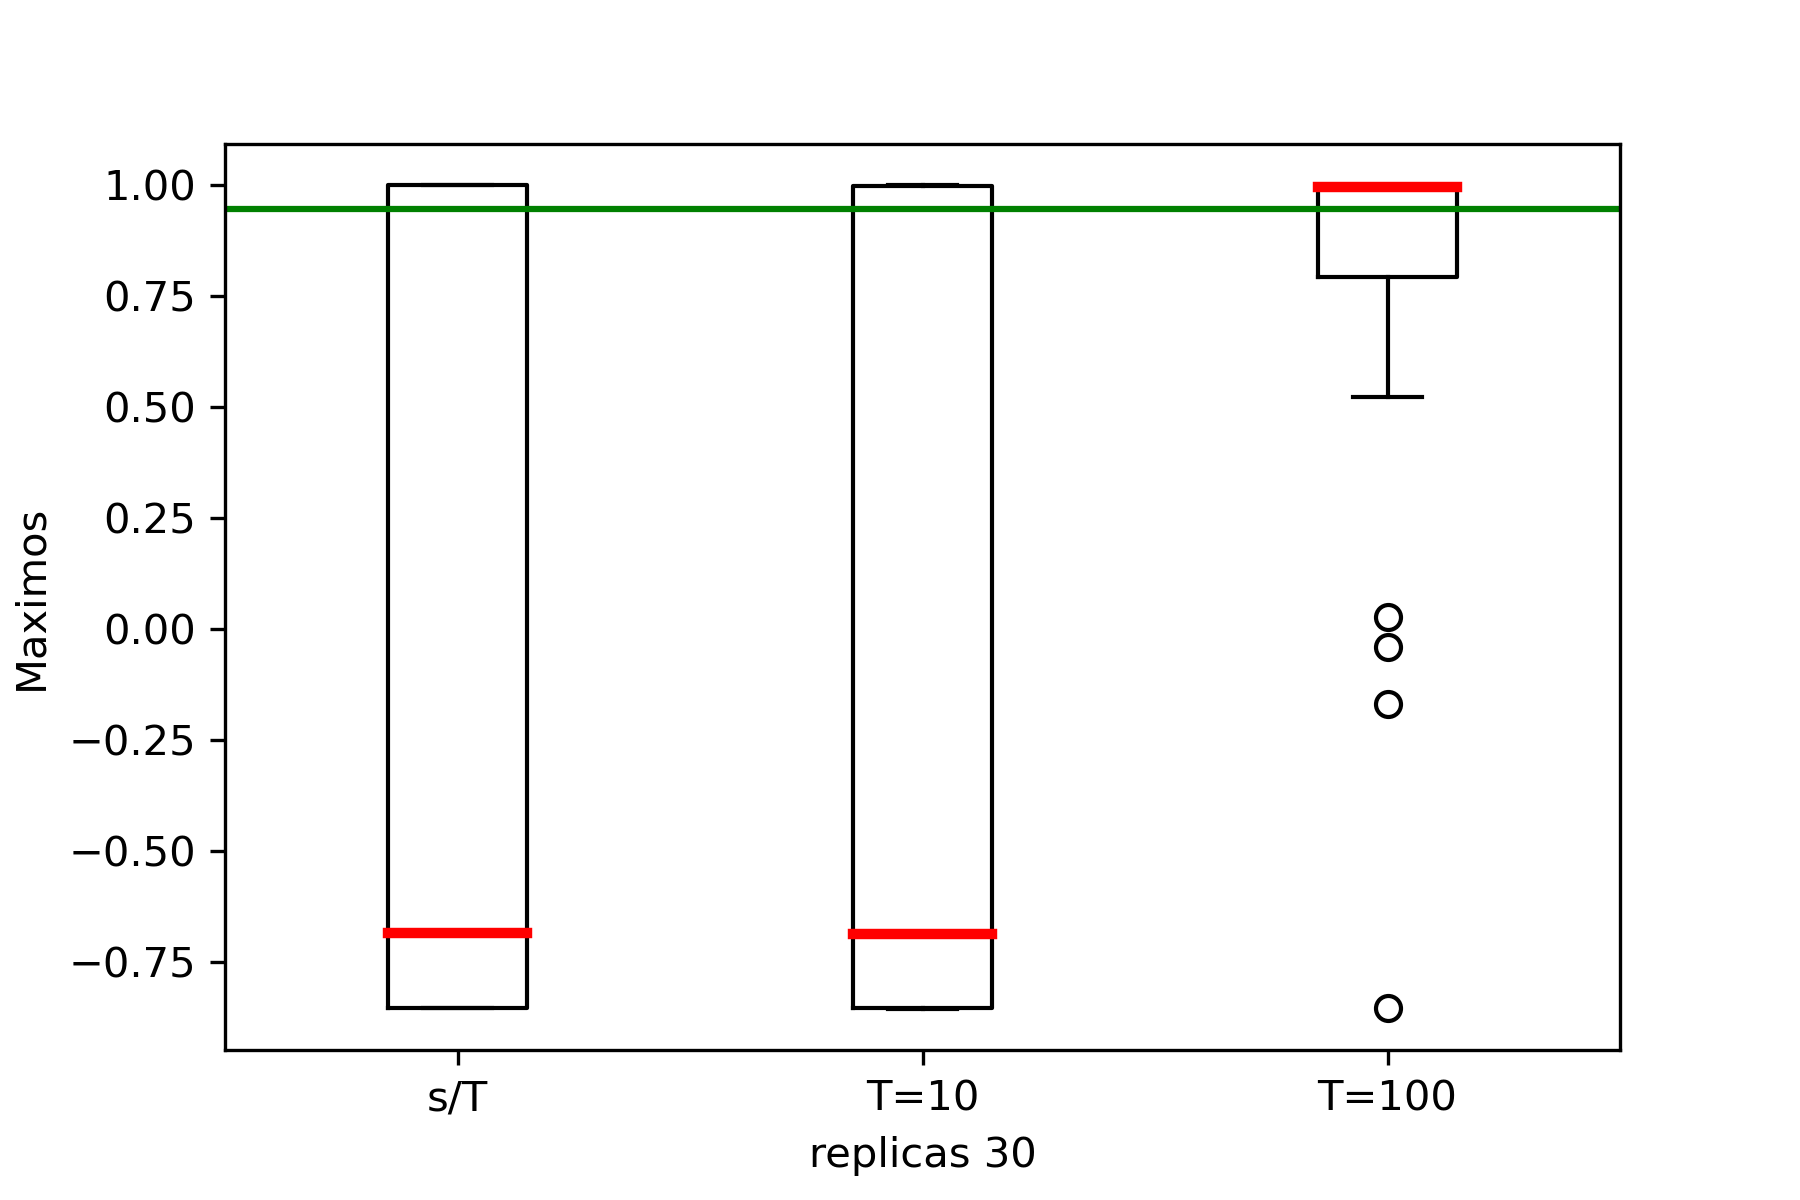
\includegraphics[width=\linewidth]{p7_p1000_r30.png}
\caption{1000 pasos.}
\end{subfigure}
\begin{subfigure}[b]{0.40\linewidth}
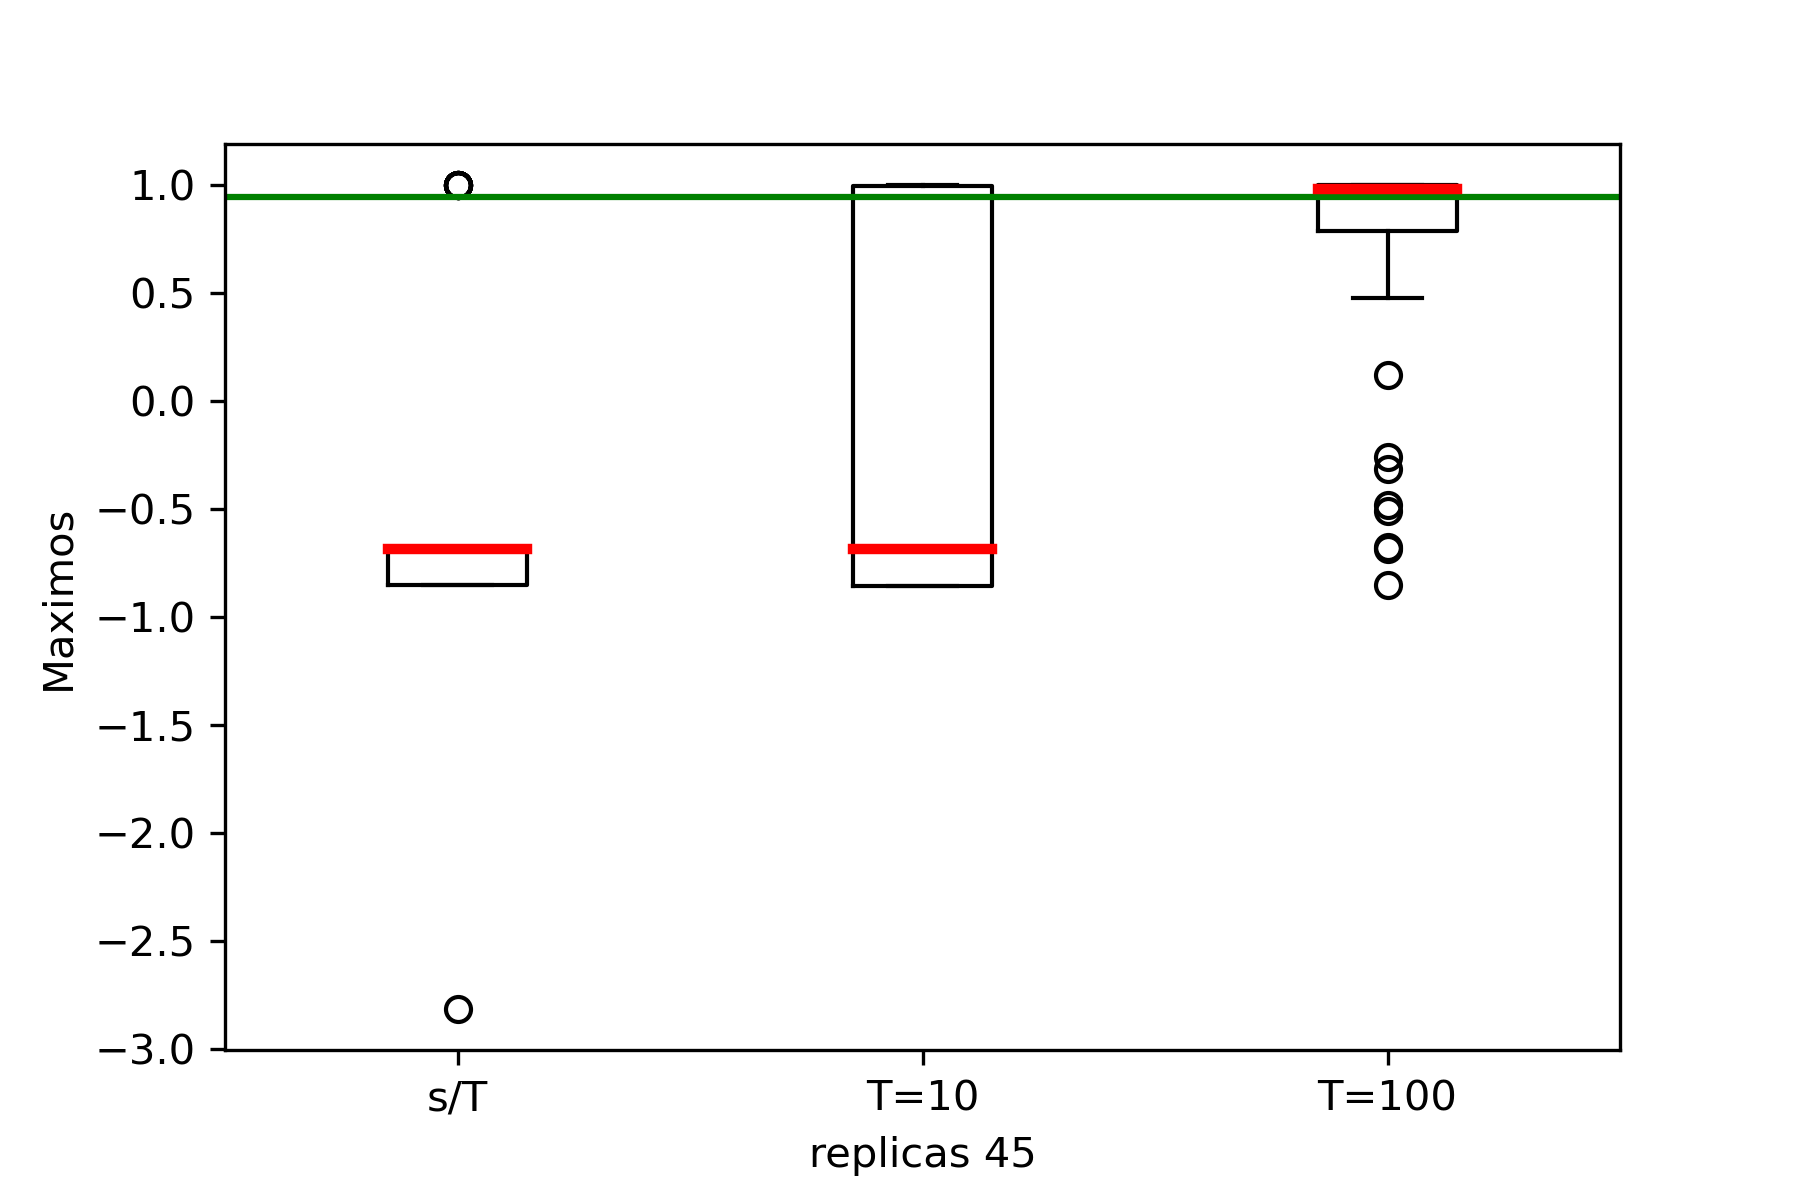
\includegraphics[width=\linewidth]{p7_p1000_r45.png}
\caption{1000 pasos.}
\end{subfigure}
\caption{Gráfica caja bigote de pasos comparando muestras sin y con temperatura y $\xi$.}
\label{fig:westminster}
\end{figure}

\begin{figure}[H]
\centering
\begin{subfigure}[b]{0.40\linewidth}
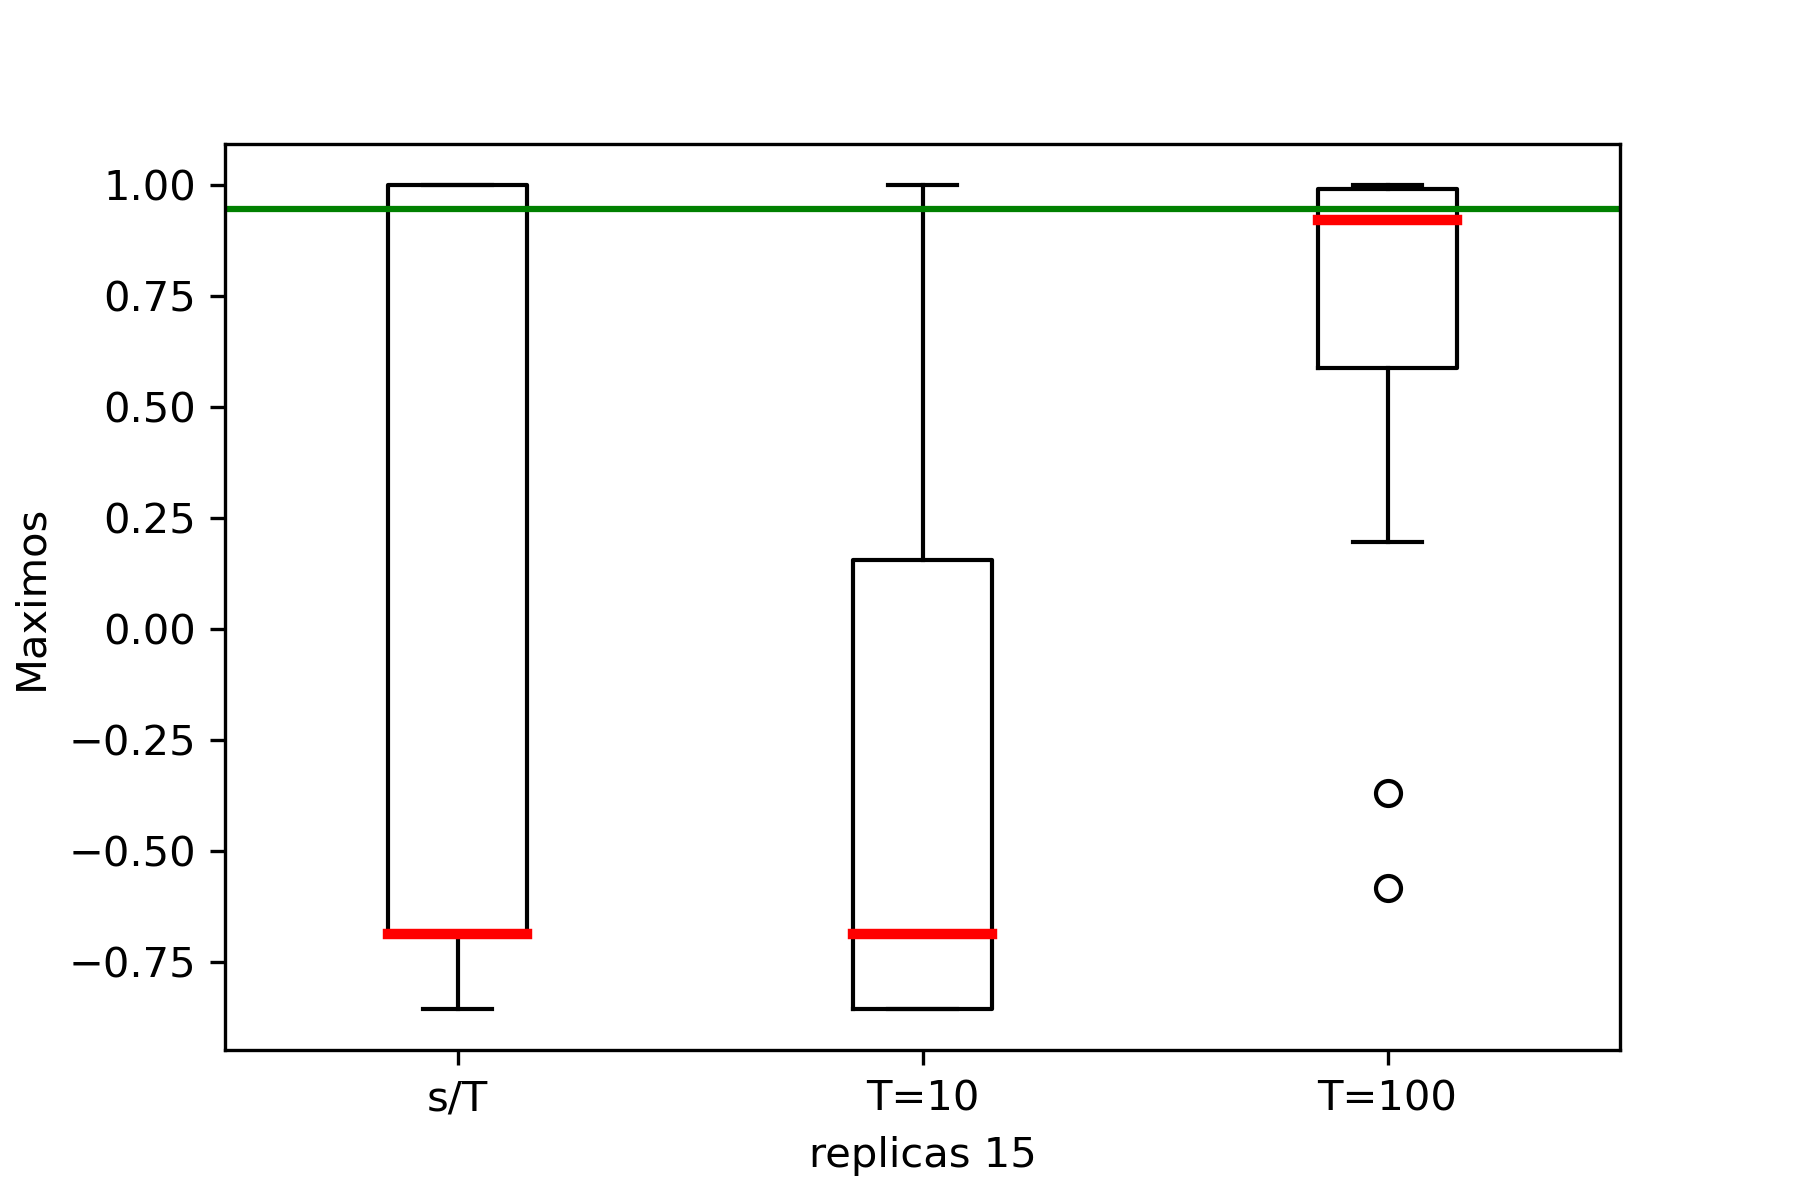
\includegraphics[width=\linewidth]{p7_p10000_r15.png}
\caption{10000 pasos.}
\end{subfigure}
\begin{subfigure}[b]{0.40\linewidth}
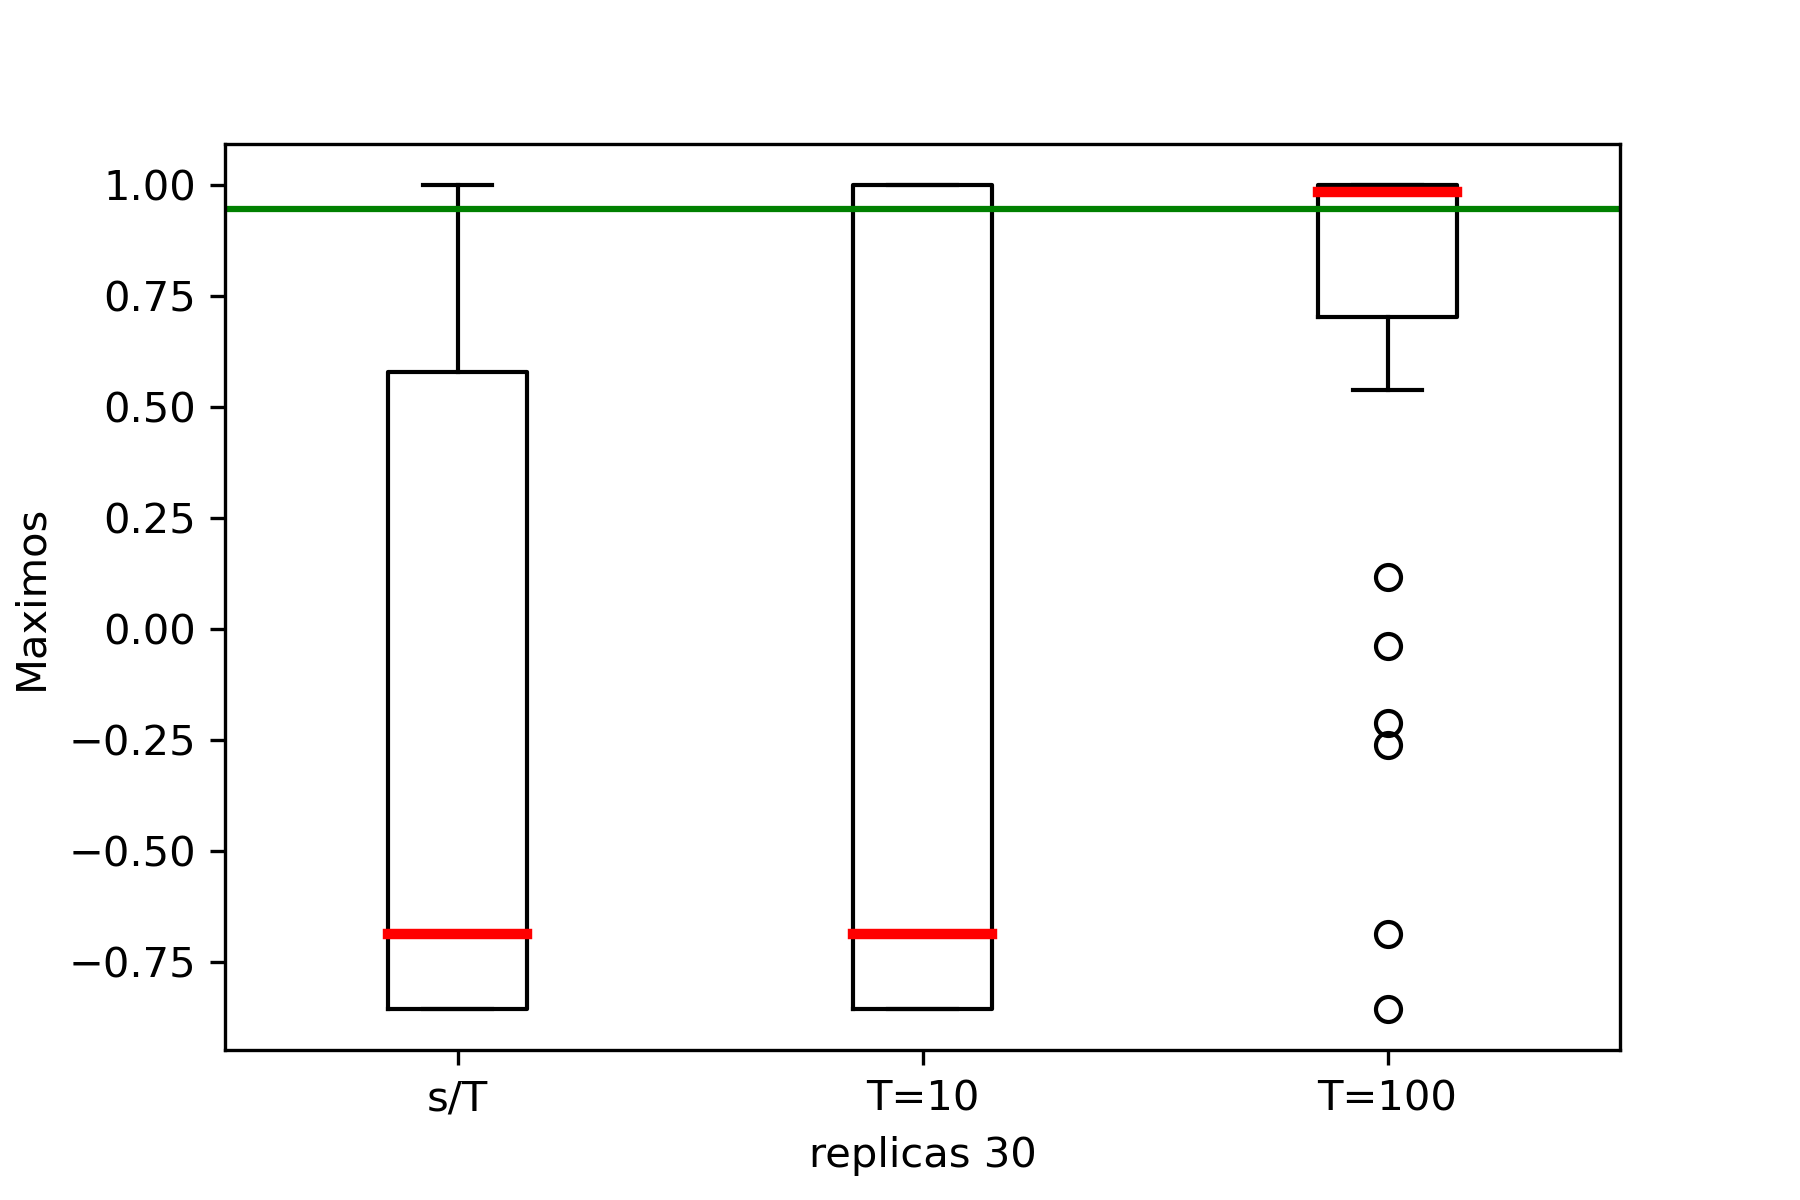
\includegraphics[width=\linewidth]{p7_p10000_r30.png}
\caption{10000 pasos.}
\end{subfigure}
\caption{Gráfica caja bigote de pasos comparando muestras sin y con temperatura y $\xi$.}
\label{fig:westminster}
\end{figure}

\begin{figure}[H]
\centering
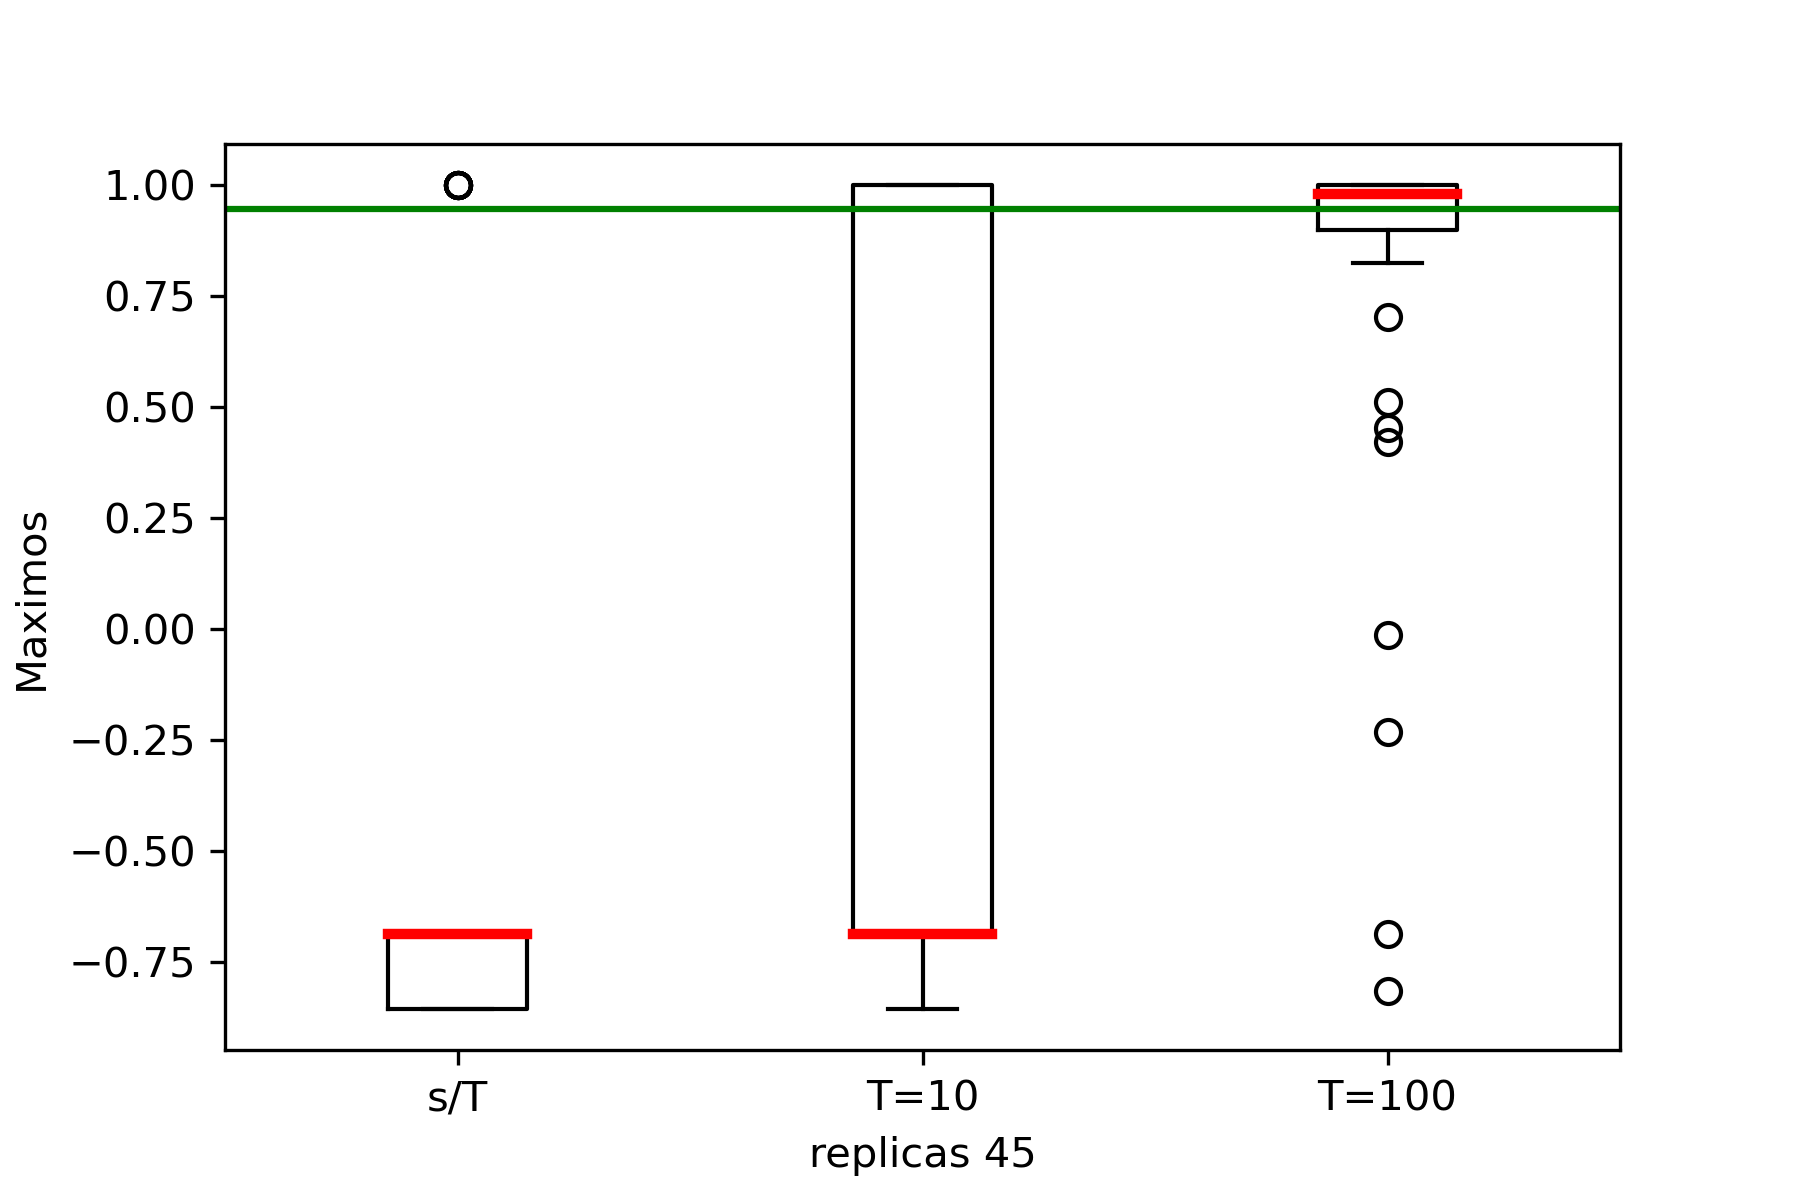
\includegraphics[width=80mm]{p7_p10000_r45.png}
\caption{\label{fig3} Gráfica caja bigote de 10000 pasos comparando muestras sin y con temperatura y $\xi$.}
\end{figure}


\printbibliography
\end{document}